\documentclass[10pt]{article}
\usepackage[margin=0.7in]{geometry}
\usepackage[T1]{fontenc}
\usepackage{lmodern,booktabs,longtable,graphicx,pdflscape,hyperref}
\pdfinfoomitdate=1
\pdftrailerid{}
\pdfsuppressptexinfo=15
\hypersetup{colorlinks=true,urlcolor=teal,linkcolor=black}
\usepackage{xcolor}
\setlength{\emergencystretch}{3em}
\title{Equity Duration and Predictability\\Replication, Update, and Sector ER Tracker}
\author{Yuting Li, Yiyao Wang, Gary Miao, and Luke Zhu}
\date{FINM 32800}
\begin{document}\maketitle
\section{Purpose and findings}
The project reproduces Golez and Koudijs (2025) and asks whether payout-related valuation decompositions persist within industries. The intended user is an equity researcher assessing whether an apparent valuation pattern reflects industry composition or unstable estimation. ER is a model-dependent expected-return contribution to log dividend-price variation, not an expected return or trading signal.

The paper-sample translation reproduces 264 independently calculated numeric cells within the committed rounding tolerance. Two historical Table 4 smoothing entries remain unrecomputed because early earnings and the upstream estimation file are absent. The postwar entry is recomputed using nominal growth; the real-growth convention is reported separately.

\subsection{Recent-data update}
Post-1945 result holds through 2025: the expected-return share is 0.89 (paper sample 0.91) and the dividend-growth share is 0.12 (paper sample 0.10). The return-predictability t-statistic is 1.69 (paper sample 2.10), so returns are no longer significantly predictable at the 5\% level on their own. Strips still have a smaller expected-return share than the market (0.77 vs 0.96; paper 0.56 vs 0.96).

The stock-level update covers 1970-2025. Low/high tercile ER equals 0.519/0.475. The ordering holds in this construction. A shorter stock-history sample and overlap discrepancies prevent describing it as an exact extension of the original stock-selection code.

\subsection{Agreed extension}
Sector ER Tracker was confirmed as the consultation-agreed extension by the team on November 18, 2026. It compares payout groups within industries, equal industry weights across sides, and market-wide sorts on common years. Annual stock formation uses established dividend payers and lagged accounting. Historical revisions make the exercise pseudo-real-time.

Industry-neutral: low-minus-high ER is 0.117, with a 95 percent paired stationary-block interval [-1.567, 3.816], using 31 annual outcomes. 
Market-wide: low-minus-high ER is -0.255, with a 95 percent paired stationary-block interval [-10.905, 6.385], using 31 annual outcomes. 

\section{Sources, construction, and limitations}
The baseline uses the authors' Mendeley version-one package. Updates use Goyal annual data, WRDS CRSP, Compustat, CCM and OptionMetrics. Historical SIC is mapped to Kenneth French industries; FRED CPI deflates annual values. Cash dividends are adjusted using daily and monthly cumulative share factors. Portfolio weights drift within each calendar year; industry sleeves are combined at identical monthly industry weights. Accounting net income and common dividends use matching issuer units. No current constituent list is imposed on history.

Cash withdrawals differ from CRSP daily dividend reinvestment. The pipeline therefore checks separate cash-event and return fields, records filter attrition and sample breaks, and avoids silently filling unavailable outcomes. Table 4 smoothing remains an identified source limitation. Earlier strip-rebuild thresholds were exploratory, not selected blind. Registered new identity and cash-validation gates apply prospectively; the report does not claim that old results were unseen.


\section{Data validation}
8 of 8 registered checks pass. The median cash-versus-effective yield gap on dividend-paying months is 0.000175; cash withdrawals and daily dividend reinvestment are different conventions. The coverage panel records observed filter attrition, not an assumed target count. A passing identity does not establish exact equivalence to the authors' stock-selection procedure.

\section{Generated results}
All numerical results, captions containing estimates, tables and figures below are generated from pipeline artifacts. The archived forecasting exercise is a sensitivity appendix, not the consultation-agreed product.

Postwar smoothing equals 0.211 using nominal growth and 0.226 using real growth, over 77 matched growth observations. The nominal convention matches the printed entry; this convention distinction remains explicit.

\begin{landscape}\small

\begin{longtable}{lrr}
\caption{Paper-sample replication: Table 1. Mean annual market return is 6.38\% versus 5.25\% for dividend strips; their different cash-flow horizons motivate the predictability comparison.} \\
\toprule
Statistic & Market & Dividend strips \\
\midrule
\endfirsthead
\caption[]{Paper-sample replication: Table 1. Mean annual market return is 6.38\% versus 5.25\% for dividend strips; their different cash-flow horizons motivate the predictability comparison.} \\
\toprule
Statistic & Market & Dividend strips \\
\midrule
\endhead
\midrule
\multicolumn{3}{r}{Continued on next page} \\
\midrule
\endfoot
\bottomrule
\endlastfoot
Return mean (\%) & 6.377 & 5.246 \\
Return SD (\%) & 17.080 & 14.216 \\
Dividend growth mean (\%) & 3.320 & -- \\
Dividend growth SD (\%) & 7.617 & -- \\
Dividend-price mean (\%) & 1.820 & 66.994 \\
Dividend-price SD (\%) & 0.376 & 9.386 \\
\end{longtable}


\end{landscape}


\begin{landscape}\small

\begin{longtable}{lrr}
\caption{Paper-sample replication: Table 2. Estimated ER ranges from 0.564 to 0.960; shares are model-dependent and are not clipped to zero or one.} \\
\toprule
Statistic & Market & Dividend strips \\
\midrule
\endfirsthead
\caption[]{Paper-sample replication: Table 2. Estimated ER ranges from 0.564 to 0.960; shares are model-dependent and are not clipped to zero or one.} \\
\toprule
Statistic & Market & Dividend strips \\
\midrule
\endhead
\midrule
\multicolumn{3}{r}{Continued on next page} \\
\midrule
\endfoot
\bottomrule
\endlastfoot
Return slope & 0.389 & 0.564 \\
Return t-stat (NW) & 3.539 & 6.613 \\
Return t-stat (non-overlap) & 2.843 & 3.399 \\
Return R-squared & 0.212 & 0.256 \\
Dividend growth slope & -0.019 & -0.399 \\
Dividend growth t-stat (NW) & -0.151 & -4.314 \\
Dividend growth t-stat (non-overlap) & -0.055 & -3.592 \\
Dividend growth R-squared & 0.003 & 0.447 \\
Dividend-price slope & 0.606 & -- \\
Dividend-price t-stat (NW) & 4.862 & -- \\
Dividend-price t-stat (non-overlap) & 4.083 & -- \\
Dividend-price R-squared & 0.370 & -- \\
ER & 0.960 & 0.564 \\
ER (implied) & 0.953 & 0.601 \\
EDG & 0.047 & 0.399 \\
EDG (implied) & 0.040 & 0.436 \\
\end{longtable}


\end{landscape}


\begin{landscape}\small

\begin{longtable}{lrrr}
\caption{Paper-sample replication: Table 4. Mean payout ranges from 47.3\% to 98.4\% across historical samples. Postwar smoothing is calculated from nominal growth; historical smoothing remains supplied or unavailable.} \\
\toprule
Statistic & 1945-2022 & 1629-1945 & 1629-2022 \\
\midrule
\endfirsthead
\caption[]{Paper-sample replication: Table 4. Mean payout ranges from 47.3\% to 98.4\% across historical samples. Postwar smoothing is calculated from nominal growth; historical smoothing remains supplied or unavailable.} \\
\toprule
Statistic & 1945-2022 & 1629-1945 & 1629-2022 \\
\midrule
\endhead
\midrule
\multicolumn{4}{r}{Continued on next page} \\
\midrule
\endfoot
\bottomrule
\endlastfoot
Payout (\%) & 47.264 & 98.410 & 86.114 \\
Return mean (\%) & 6.560 & 5.864 & 6.001 \\
Return SD (\%) & 16.910 & 14.122 & 14.692 \\
DY/RET & 0.406 & 0.688 & 0.625 \\
Dividend growth mean (\%) & 2.373 & 0.809 & 1.117 \\
Dividend growth SD (\%) & 6.674 & 13.291 & 12.281 \\
Dividend-price mean (\%) & 3.242 & 4.856 & 4.539 \\
Dividend-price SD (\%) & 1.426 & 1.271 & 1.453 \\
Dividend-price AR(1) & 0.905 & 0.694 & 0.790 \\
Smoothing* & 0.211 & 0.320 & 0.310 \\
\end{longtable}


\end{landscape}


\begin{landscape}\small

\begin{longtable}{lrrr}
\caption{Paper-sample replication: Table 5. Estimated ER ranges from 0.343 to 0.909; shares are model-dependent and are not clipped to zero or one.} \\
\toprule
Statistic & 1945-2022 & 1629-1945 & 1629-2022 \\
\midrule
\endfirsthead
\caption[]{Paper-sample replication: Table 5. Estimated ER ranges from 0.343 to 0.909; shares are model-dependent and are not clipped to zero or one.} \\
\toprule
Statistic & 1945-2022 & 1629-1945 & 1629-2022 \\
\midrule
\endhead
\midrule
\multicolumn{4}{r}{Continued on next page} \\
\midrule
\endfoot
\bottomrule
\endlastfoot
Return slope & 0.086 & 0.109 & 0.067 \\
Return t-stat (NW) & 2.105 & 3.225 & 2.703 \\
Return difference t-stat & -- & 0.420 & -- \\
Return R-squared & 0.053 & 0.036 & 0.026 \\
Dividend growth slope & -0.009 & -0.198 & -0.092 \\
Dividend growth t-stat (NW) & -0.408 & -5.298 & -4.137 \\
Dividend growth difference t-stat & -- & -4.291 & -- \\
Dividend growth R-squared & 0.004 & 0.136 & 0.069 \\
Dividend-price slope & 0.932 & 0.715 & 0.869 \\
Dividend-price t-stat (NW) & 21.748 & 15.745 & 27.792 \\
Dividend-price difference t-stat & -- & -3.462 & -- \\
Dividend-price R-squared & 0.856 & 0.521 & 0.750 \\
ER & 0.909 & 0.343 & 0.403 \\
ER (implied) & 0.901 & 0.375 & 0.450 \\
EDG & 0.099 & 0.625 & 0.550 \\
EDG (implied) & 0.091 & 0.657 & 0.597 \\
\end{longtable}


\end{landscape}


\begin{landscape}\small

\begin{longtable}{lrrrrrr}
\caption{Paper-sample replication: Table 6. Mean portfolio payout ranges from 31.6\% to 64.2\%; the portfolio sorts therefore create variation in the paper's duration proxy. Missing earnings constrain payout and smoothing summaries.} \\
\toprule
Statistic & All & Low & Medium & High & Below 0.5 & Above 0.5 \\
\midrule
\endfirsthead
\caption[]{Paper-sample replication: Table 6. Mean portfolio payout ranges from 31.6\% to 64.2\%; the portfolio sorts therefore create variation in the paper's duration proxy. Missing earnings constrain payout and smoothing summaries.} \\
\toprule
Statistic & All & Low & Medium & High & Below 0.5 & Above 0.5 \\
\midrule
\endhead
\midrule
\multicolumn{7}{r}{Continued on next page} \\
\midrule
\endfoot
\bottomrule
\endlastfoot
Number of stocks: mean & 724.782 & 241.244 & 241.974 & 241.564 & 445.590 & 279.192 \\
Number of stocks: min & 206.000 & 68.000 & 69.000 & 69.000 & 12.000 & 155.000 \\
Number of stocks: max & 1211.000 & 403.000 & 404.000 & 404.000 & 951.000 & 409.000 \\
Payout (\%) & 48.698 & 31.602 & 47.541 & 64.183 & 39.875 & 63.343 \\
Return mean (\%) & 6.488 & 6.788 & 6.780 & 5.786 & 6.966 & 6.283 \\
Return SD (\%) & 15.392 & 17.833 & 15.746 & 14.341 & 16.950 & 14.242 \\
DY/RET & 0.453 & 0.294 & 0.419 & 0.633 & 0.356 & 0.590 \\
Dividend growth mean (\%) & 2.356 & 3.165 & 2.779 & 1.132 & 3.081 & 1.729 \\
Dividend growth SD (\%) & 6.292 & 9.230 & 6.010 & 9.031 & 7.064 & 7.794 \\
Dividend-price mean (\%) & 3.482 & 2.436 & 3.366 & 4.379 & 2.976 & 4.364 \\
Dividend-price SD (\%) & 1.255 & 1.289 & 1.155 & 1.354 & 1.262 & 1.490 \\
Dividend-price AR(1) & 0.881 & 0.910 & 0.868 & 0.842 & 0.882 & 0.875 \\
Smoothing & 0.322 & 0.501 & 0.308 & 0.176 & 0.421 & 0.145 \\
\end{longtable}


\end{landscape}


\begin{landscape}\small

\begin{longtable}{lrrrrrr}
\caption{Paper-sample replication: Table 7. Estimated ER ranges from 0.541 to 1.041; shares are model-dependent and are not clipped to zero or one.} \\
\toprule
Statistic & All & Low & Medium & High & Below 0.5 & Above 0.5 \\
\midrule
\endfirsthead
\caption[]{Paper-sample replication: Table 7. Estimated ER ranges from 0.541 to 1.041; shares are model-dependent and are not clipped to zero or one.} \\
\toprule
Statistic & All & Low & Medium & High & Below 0.5 & Above 0.5 \\
\midrule
\endhead
\midrule
\multicolumn{7}{r}{Continued on next page} \\
\midrule
\endfoot
\bottomrule
\endlastfoot
Return slope & 0.099 & 0.093 & 0.105 & 0.088 & 0.114 & 0.085 \\
Return t-stat (NW) & 2.439 & 2.385 & 2.494 & 1.970 & 2.618 & 1.770 \\
Return R-squared & 0.053 & 0.069 & 0.052 & 0.035 & 0.075 & 0.037 \\
Dividend growth slope & -0.020 & 0.001 & -0.027 & -0.076 & -0.002 & -0.062 \\
Dividend growth t-stat (NW) & -0.851 & 0.061 & -1.225 & -1.944 & -0.111 & -1.971 \\
Dividend growth R-squared & 0.013 & 0.000 & 0.024 & 0.066 & 0.000 & 0.066 \\
Dividend-price slope & 0.911 & 0.930 & 0.896 & 0.873 & 0.910 & 0.892 \\
Dividend-price t-stat (NW) & 20.778 & 21.905 & 19.395 & 14.983 & 21.195 & 17.850 \\
Dividend-price R-squared & 0.816 & 0.864 & 0.790 & 0.750 & 0.816 & 0.786 \\
ER & 0.839 & 1.041 & 0.800 & 0.541 & 1.000 & 0.591 \\
ER (implied) & 0.830 & 1.015 & 0.794 & 0.534 & 0.981 & 0.570 \\
EDG & 0.170 & -0.015 & 0.206 & 0.466 & 0.019 & 0.430 \\
EDG (implied) & 0.161 & -0.041 & 0.200 & 0.459 & 0.000 & 0.409 \\
\end{longtable}


\end{landscape}


\begin{landscape}\small

\begin{longtable}{lrr}
\caption{Updated data: Table 1. Mean annual market return is 6.97\% versus 8.44\% for dividend strips; their different cash-flow horizons motivate the predictability comparison.} \\
\toprule
Statistic & Market & Dividend strips \\
\midrule
\endfirsthead
\caption[]{Updated data: Table 1. Mean annual market return is 6.97\% versus 8.44\% for dividend strips; their different cash-flow horizons motivate the predictability comparison.} \\
\toprule
Statistic & Market & Dividend strips \\
\midrule
\endhead
\midrule
\multicolumn{3}{r}{Continued on next page} \\
\midrule
\endfoot
\bottomrule
\endlastfoot
Return mean (\%) & 6.974 & 8.442 \\
Return SD (\%) & 16.726 & 18.810 \\
Dividend growth mean (\%) & 3.303 & -- \\
Dividend growth SD (\%) & 7.263 & -- \\
Dividend-price mean (\%) & 1.784 & 70.314 \\
Dividend-price SD (\%) & 0.380 & 15.334 \\
\end{longtable}


\end{landscape}


\begin{landscape}\small

\begin{longtable}{lrr}
\caption{Updated data: Table 2. Estimated ER ranges from 0.770 to 0.956; shares are model-dependent and are not clipped to zero or one.} \\
\toprule
Statistic & Market & Dividend strips \\
\midrule
\endfirsthead
\caption[]{Updated data: Table 2. Estimated ER ranges from 0.770 to 0.956; shares are model-dependent and are not clipped to zero or one.} \\
\toprule
Statistic & Market & Dividend strips \\
\midrule
\endhead
\midrule
\multicolumn{3}{r}{Continued on next page} \\
\midrule
\endfoot
\bottomrule
\endlastfoot
Return slope & 0.349 & 0.770 \\
Return t-stat (NW) & 3.176 & 7.709 \\
Return t-stat (non-overlap) & 2.566 & 5.068 \\
Return R-squared & 0.175 & 0.451 \\
Dividend growth slope & -0.018 & -0.224 \\
Dividend growth t-stat (NW) & -0.150 & -2.475 \\
Dividend growth t-stat (non-overlap) & -0.060 & -2.189 \\
Dividend growth R-squared & 0.002 & 0.256 \\
Dividend-price slope & 0.646 & -- \\
Dividend-price t-stat (NW) & 5.394 & -- \\
Dividend-price t-stat (non-overlap) & 4.587 & -- \\
Dividend-price R-squared & 0.396 & -- \\
ER & 0.956 & 0.770 \\
ER (implied) & 0.952 & 0.776 \\
EDG & 0.048 & 0.224 \\
EDG (implied) & 0.044 & 0.230 \\
\end{longtable}


\end{landscape}


\begin{landscape}\small

\begin{longtable}{lrrr}
\caption{Updated data: Table 4. Mean payout ranges from 47.0\% to 98.4\% across historical samples. Postwar smoothing is calculated from nominal growth; historical smoothing remains supplied or unavailable.} \\
\toprule
Statistic & 1945-2025 & 1629-1945 & 1629-2025 \\
\midrule
\endfirsthead
\caption[]{Updated data: Table 4. Mean payout ranges from 47.0\% to 98.4\% across historical samples. Postwar smoothing is calculated from nominal growth; historical smoothing remains supplied or unavailable.} \\
\toprule
Statistic & 1945-2025 & 1629-1945 & 1629-2025 \\
\midrule
\endhead
\midrule
\multicolumn{4}{r}{Continued on next page} \\
\midrule
\endfoot
\bottomrule
\endlastfoot
Payout (\%) & 46.970 & 98.410 & 85.639 \\
Return mean (\%) & 6.975 & 5.864 & 6.089 \\
Return SD (\%) & 16.730 & 14.122 & 14.673 \\
DY/RET & 0.379 & 0.688 & 0.614 \\
Dividend growth mean (\%) & 2.381 & 0.809 & 1.128 \\
Dividend growth SD (\%) & 6.548 & 13.291 & 12.235 \\
Dividend-price mean (\%) & 3.170 & 4.856 & 4.514 \\
Dividend-price SD (\%) & 1.447 & 1.271 & 1.474 \\
Dividend-price AR(1) & 0.905 & 0.694 & 0.795 \\
Smoothing* & 0.211 & 0.320 & -- \\
\end{longtable}


\end{landscape}


\begin{landscape}\small

\begin{longtable}{lrrr}
\caption{Updated data: Table 5. Estimated ER ranges from 0.343 to 0.893; shares are model-dependent and are not clipped to zero or one.} \\
\toprule
Statistic & 1945-2025 & 1629-1945 & 1629-2025 \\
\midrule
\endfirsthead
\caption[]{Updated data: Table 5. Estimated ER ranges from 0.343 to 0.893; shares are model-dependent and are not clipped to zero or one.} \\
\toprule
Statistic & 1945-2025 & 1629-1945 & 1629-2025 \\
\midrule
\endhead
\midrule
\multicolumn{4}{r}{Continued on next page} \\
\midrule
\endfoot
\bottomrule
\endlastfoot
Return slope & 0.066 & 0.109 & 0.056 \\
Return t-stat (NW) & 1.690 & 3.225 & 2.326 \\
Return difference t-stat & -- & 0.813 & -- \\
Return R-squared & 0.034 & 0.036 & 0.019 \\
Dividend growth slope & -0.009 & -0.198 & -0.087 \\
Dividend growth t-stat (NW) & -0.420 & -5.298 & -4.152 \\
Dividend growth difference t-stat & -- & -4.390 & -- \\
Dividend growth R-squared & 0.004 & 0.136 & 0.065 \\
Dividend-price slope & 0.952 & 0.715 & 0.886 \\
Dividend-price t-stat (NW) & 23.426 & 15.745 & 29.223 \\
Dividend-price difference t-stat & -- & -3.878 & -- \\
Dividend-price R-squared & 0.868 & 0.521 & 0.766 \\
ER & 0.893 & 0.343 & 0.371 \\
ER (implied) & 0.880 & 0.375 & 0.424 \\
EDG & 0.120 & 0.625 & 0.576 \\
EDG (implied) & 0.107 & 0.657 & 0.629 \\
\end{longtable}


\end{landscape}


\begin{landscape}\small

\begin{longtable}{lrrrrrr}
\caption{Updated data: Table 6. Mean portfolio payout ranges from 29.7\% to 63.5\%; the portfolio sorts therefore create variation in the paper's duration proxy. Missing earnings constrain payout and smoothing summaries.} \\
\toprule
Statistic & All & Low & Medium & High & Below 0.5 & Above 0.5 \\
\midrule
\endfirsthead
\caption[]{Updated data: Table 6. Mean portfolio payout ranges from 29.7\% to 63.5\%; the portfolio sorts therefore create variation in the paper's duration proxy. Missing earnings constrain payout and smoothing summaries.} \\
\toprule
Statistic & All & Low & Medium & High & Below 0.5 & Above 0.5 \\
\midrule
\endhead
\midrule
\multicolumn{7}{r}{Continued on next page} \\
\midrule
\endfoot
\bottomrule
\endlastfoot
Number of stocks: mean & 840.357 & 281.446 & 279.214 & 279.696 & 572.179 & 268.179 \\
Number of stocks: min & 415.000 & 139.000 & 138.000 & 138.000 & 227.000 & 153.000 \\
Number of stocks: max & 1228.000 & 405.000 & 413.000 & 410.000 & 1033.000 & 400.000 \\
Payout (\%) & 46.820 & 29.690 & 46.610 & 62.917 & 39.337 & 63.531 \\
Return mean (\%) & 6.687 & 6.754 & 6.862 & 6.136 & 6.889 & 6.385 \\
Return SD (\%) & 15.267 & 18.014 & 16.196 & 13.542 & 16.767 & 13.631 \\
DY/RET & 0.378 & 0.213 & 0.353 & 0.557 & 0.300 & 0.545 \\
Dividend growth mean (\%) & 2.319 & 2.956 & 2.508 & 1.547 & 2.636 & 1.848 \\
Dividend growth SD (\%) & 5.737 & 8.736 & 6.450 & 6.944 & 7.602 & 6.168 \\
Dividend-price mean (\%) & 2.973 & 1.766 & 2.878 & 3.972 & 2.477 & 4.019 \\
Dividend-price SD (\%) & 1.086 & 0.714 & 0.965 & 1.265 & 0.984 & 1.390 \\
Dividend-price AR(1) & 0.860 & 0.814 & 0.832 & 0.852 & 0.852 & 0.894 \\
Smoothing & 0.205 & 0.429 & 0.232 & 0.173 & 0.310 & 0.126 \\
\end{longtable}


\end{landscape}


\begin{landscape}\small

\begin{longtable}{lrrrrrr}
\caption{Updated data: Table 7. Estimated ER ranges from 0.475 to 0.777; shares are model-dependent and are not clipped to zero or one.} \\
\toprule
Statistic & All & Low & Medium & High & Below 0.5 & Above 0.5 \\
\midrule
\endfirsthead
\caption[]{Updated data: Table 7. Estimated ER ranges from 0.475 to 0.777; shares are model-dependent and are not clipped to zero or one.} \\
\toprule
Statistic & All & Low & Medium & High & Below 0.5 & Above 0.5 \\
\midrule
\endhead
\midrule
\multicolumn{7}{r}{Continued on next page} \\
\midrule
\endfoot
\bottomrule
\endlastfoot
Return slope & 0.060 & 0.063 & 0.100 & 0.071 & 0.065 & 0.062 \\
Return t-stat (NW) & 1.255 & 1.218 & 1.975 & 1.244 & 1.381 & 1.157 \\
Return R-squared & 0.018 & 0.019 & 0.039 & 0.025 & 0.021 & 0.022 \\
Dividend growth slope & -0.052 & -0.058 & -0.030 & -0.081 & -0.040 & -0.063 \\
Dividend growth t-stat (NW) & -2.732 & -2.166 & -1.432 & -2.631 & -1.618 & -2.520 \\
Dividend growth R-squared & 0.096 & 0.071 & 0.022 & 0.125 & 0.039 & 0.112 \\
Dividend-price slope & 0.915 & 0.894 & 0.895 & 0.882 & 0.917 & 0.911 \\
Dividend-price t-stat (NW) & 17.215 & 13.850 & 16.071 & 13.946 & 15.858 & 18.285 \\
Dividend-price R-squared & 0.792 & 0.745 & 0.754 & 0.762 & 0.775 & 0.815 \\
ER & 0.547 & 0.519 & 0.777 & 0.475 & 0.630 & 0.509 \\
ER (implied) & 0.529 & 0.516 & 0.766 & 0.459 & 0.614 & 0.483 \\
EDG & 0.471 & 0.484 & 0.234 & 0.541 & 0.386 & 0.517 \\
EDG (implied) & 0.453 & 0.481 & 0.223 & 0.525 & 0.370 & 0.491 \\
\end{longtable}


\end{landscape}


\begin{landscape}\small

\begin{longtable}{lrrrrrr}
\caption{Common-period author common: Table 6. Differences isolate construction from the change in sample endpoint.} \\
\toprule
Statistic & All & Low & Medium & High & Below 0.5 & Above 0.5 \\
\midrule
\endfirsthead
\caption[]{Common-period author common: Table 6. Differences isolate construction from the change in sample endpoint.} \\
\toprule
Statistic & All & Low & Medium & High & Below 0.5 & Above 0.5 \\
\midrule
\endhead
\midrule
\multicolumn{7}{r}{Continued on next page} \\
\midrule
\endfoot
\bottomrule
\endlastfoot
Number of stocks: mean & 849.528 & 282.830 & 283.547 & 283.151 & 573.660 & 275.868 \\
Number of stocks: min & 497.000 & 165.000 & 166.000 & 166.000 & 224.000 & 155.000 \\
Number of stocks: max & 1211.000 & 403.000 & 404.000 & 404.000 & 951.000 & 409.000 \\
Payout (\%) & 46.032 & 25.855 & 44.617 & 64.507 & 37.700 & 65.067 \\
Return mean (\%) & 6.022 & 5.547 & 6.790 & 5.550 & 6.055 & 6.060 \\
Return SD (\%) & 15.431 & 17.990 & 16.094 & 14.037 & 16.810 & 14.121 \\
DY/RET & 0.436 & 0.261 & 0.373 & 0.640 & 0.350 & 0.604 \\
Dividend growth mean (\%) & 1.952 & 2.480 & 2.941 & 0.600 & 2.437 & 1.222 \\
Dividend growth SD (\%) & 6.179 & 10.161 & 5.383 & 9.037 & 7.572 & 7.753 \\
Dividend-price mean (\%) & 3.160 & 1.861 & 3.016 & 4.256 & 2.603 & 4.329 \\
Dividend-price SD (\%) & 1.166 & 0.729 & 1.033 & 1.435 & 1.019 & 1.651 \\
Dividend-price AR(1) & 0.874 & 0.830 & 0.851 & 0.852 & 0.867 & 0.889 \\
Smoothing & 0.284 & 0.509 & 0.272 & 0.147 & 0.424 & 0.120 \\
\end{longtable}


\end{landscape}


\begin{landscape}\small

\begin{longtable}{lrrrrrr}
\caption{Common-period author common: Table 7. Differences isolate construction from the change in sample endpoint.} \\
\toprule
Statistic & All & Low & Medium & High & Below 0.5 & Above 0.5 \\
\midrule
\endfirsthead
\caption[]{Common-period author common: Table 7. Differences isolate construction from the change in sample endpoint.} \\
\toprule
Statistic & All & Low & Medium & High & Below 0.5 & Above 0.5 \\
\midrule
\endhead
\midrule
\multicolumn{7}{r}{Continued on next page} \\
\midrule
\endfoot
\bottomrule
\endlastfoot
Return slope & 0.073 & 0.074 & 0.102 & 0.063 & 0.087 & 0.055 \\
Return t-stat (NW) & 1.571 & 1.421 & 2.021 & 1.198 & 1.779 & 1.013 \\
Return R-squared & 0.029 & 0.028 & 0.045 & 0.022 & 0.038 & 0.019 \\
Dividend growth slope & -0.051 & -0.060 & -0.044 & -0.091 & -0.041 & -0.075 \\
Dividend growth t-stat (NW) & -2.551 & -2.037 & -2.593 & -2.288 & -1.781 & -2.437 \\
Dividend growth R-squared & 0.089 & 0.056 & 0.073 & 0.111 & 0.041 & 0.121 \\
Dividend-price slope & 0.904 & 0.881 & 0.880 & 0.882 & 0.895 & 0.909 \\
Dividend-price t-stat (NW) & 18.070 & 14.951 & 16.125 & 12.995 & 17.955 & 16.310 \\
Dividend-price R-squared & 0.808 & 0.782 & 0.766 & 0.768 & 0.789 & 0.816 \\
ER & 0.595 & 0.554 & 0.708 & 0.414 & 0.691 & 0.433 \\
ER (implied) & 0.580 & 0.555 & 0.697 & 0.403 & 0.677 & 0.403 \\
EDG & 0.420 & 0.445 & 0.303 & 0.597 & 0.323 & 0.597 \\
EDG (implied) & 0.405 & 0.446 & 0.292 & 0.586 & 0.309 & 0.567 \\
\end{longtable}


\end{landscape}


\begin{landscape}\small

\begin{longtable}{lrrrrrr}
\caption{Common-period rebuild common: Table 6. Differences isolate construction from the change in sample endpoint.} \\
\toprule
Statistic & All & Low & Medium & High & Below 0.5 & Above 0.5 \\
\midrule
\endfirsthead
\caption[]{Common-period rebuild common: Table 6. Differences isolate construction from the change in sample endpoint.} \\
\toprule
Statistic & All & Low & Medium & High & Below 0.5 & Above 0.5 \\
\midrule
\endhead
\midrule
\multicolumn{7}{r}{Continued on next page} \\
\midrule
\endfoot
\bottomrule
\endlastfoot
Number of stocks: mean & 842.113 & 282.019 & 279.717 & 280.377 & 574.113 & 268.000 \\
Number of stocks: min & 415.000 & 139.000 & 138.000 & 138.000 & 227.000 & 153.000 \\
Number of stocks: max & 1228.000 & 405.000 & 413.000 & 410.000 & 1033.000 & 400.000 \\
Payout (\%) & 46.832 & 29.715 & 46.537 & 61.991 & 39.474 & 62.894 \\
Return mean (\%) & 6.203 & 5.802 & 6.529 & 6.091 & 6.204 & 6.343 \\
Return SD (\%) & 15.562 & 18.023 & 16.584 & 13.868 & 16.971 & 13.958 \\
DY/RET & 0.411 & 0.247 & 0.374 & 0.566 & 0.336 & 0.553 \\
Dividend growth mean (\%) & 2.479 & 3.562 & 2.679 & 1.509 & 2.965 & 1.780 \\
Dividend growth SD (\%) & 5.715 & 8.070 & 6.534 & 7.123 & 7.481 & 6.286 \\
Dividend-price mean (\%) & 3.048 & 1.817 & 2.951 & 4.034 & 2.551 & 4.085 \\
Dividend-price SD (\%) & 1.067 & 0.699 & 0.940 & 1.271 & 0.959 & 1.399 \\
Dividend-price AR(1) & 0.862 & 0.827 & 0.828 & 0.847 & 0.857 & 0.890 \\
Smoothing & 0.189 & 0.370 & 0.225 & 0.173 & 0.277 & 0.124 \\
\end{longtable}


\end{landscape}


\begin{landscape}\small

\begin{longtable}{lrrrrrr}
\caption{Common-period rebuild common: Table 7. Differences isolate construction from the change in sample endpoint.} \\
\toprule
Statistic & All & Low & Medium & High & Below 0.5 & Above 0.5 \\
\midrule
\endfirsthead
\caption[]{Common-period rebuild common: Table 7. Differences isolate construction from the change in sample endpoint.} \\
\toprule
Statistic & All & Low & Medium & High & Below 0.5 & Above 0.5 \\
\midrule
\endhead
\midrule
\multicolumn{7}{r}{Continued on next page} \\
\midrule
\endfoot
\bottomrule
\endlastfoot
Return slope & 0.084 & 0.089 & 0.129 & 0.076 & 0.099 & 0.066 \\
Return t-stat (NW) & 1.699 & 1.710 & 2.253 & 1.290 & 1.975 & 1.193 \\
Return R-squared & 0.033 & 0.037 & 0.056 & 0.028 & 0.044 & 0.024 \\
Dividend growth slope & -0.059 & -0.066 & -0.041 & -0.084 & -0.052 & -0.064 \\
Dividend growth t-stat (NW) & -2.946 & -2.225 & -1.867 & -2.616 & -1.996 & -2.487 \\
Dividend growth R-squared & 0.122 & 0.102 & 0.038 & 0.127 & 0.063 & 0.111 \\
Dividend-price slope & 0.883 & 0.860 & 0.855 & 0.875 & 0.871 & 0.906 \\
Dividend-price t-stat (NW) & 16.131 & 13.045 & 14.524 & 13.253 & 14.762 & 17.383 \\
Dividend-price R-squared & 0.775 & 0.746 & 0.722 & 0.752 & 0.754 & 0.807 \\
ER & 0.595 & 0.575 & 0.764 & 0.482 & 0.663 & 0.520 \\
ER (implied) & 0.582 & 0.574 & 0.754 & 0.470 & 0.651 & 0.499 \\
EDG & 0.418 & 0.426 & 0.246 & 0.530 & 0.349 & 0.501 \\
EDG (implied) & 0.405 & 0.425 & 0.236 & 0.518 & 0.337 & 0.480 \\
\end{longtable}


\end{landscape}


\begin{landscape}\small

\begin{longtable}{lllr}
\caption{Data validation. Each registered numerical gate is evaluated on observed data; failures are retained and halt acceptance.} \\
\toprule
check & observed & tolerance & passed \\
\midrule
\endfirsthead
\caption[]{Data validation. Each registered numerical gate is evaluated on observed data; failures are retained and halt acceptance.} \\
\toprule
check & observed & tolerance & passed \\
\midrule
\endhead
\midrule
\multicolumn{4}{r}{Continued on next page} \\
\midrule
\endfoot
\bottomrule
\endlastfoot
Inflation reconciles with CPI & 0 & 1e-10 & True \\
Author tercile counts sum to all & 0 & 0 & True \\
Clean stock-month duplicate keys & 0 & 0 & True \\
Cash event matching failure fraction & 0.00022 & 0.001 & True \\
Portfolio weights sum to one & 6.66e-16 & 1e-10 & True \\
Monthly cash return identity & 2.78e-17 & 1e-10 & True \\
Cash versus effective yield: paying months & 0.000175 & 0.001 & True \\
Unexplained annual omissions & 0 & 0 & True \\
\end{longtable}


\end{landscape}


\begin{landscape}\small

\begin{longtable}{lrrrrrrrr}
\caption{Independent portfolio overlap. Correlations and stock-count ratios show remaining construction differences; this is not an exact-match acceptance claim.} \\
\toprule
portfolio & years & first\_year & last\_year & dp\_correlation & return\_correlation & growth\_correlation & missing\_rebuilt\_earnings\_years & mean\_firm\_count\_ratio \\
\midrule
\endfirsthead
\caption[]{Independent portfolio overlap. Correlations and stock-count ratios show remaining construction differences; this is not an exact-match acceptance claim.} \\
\toprule
portfolio & years & first\_year & last\_year & dp\_correlation & return\_correlation & growth\_correlation & missing\_rebuilt\_earnings\_years & mean\_firm\_count\_ratio \\
\midrule
\endhead
\midrule
\multicolumn{9}{r}{Continued on next page} \\
\midrule
\endfoot
\bottomrule
\endlastfoot
All & 53 & 1970 & 2022 & 0.996 & 0.999 & 0.870 & 0 & 0.989 \\
Low & 53 & 1970 & 2022 & 0.978 & 0.992 & 0.309 & 3 & 0.995 \\
Medium & 53 & 1970 & 2022 & 0.989 & 0.993 & 0.663 & 0 & 0.985 \\
High & 53 & 1970 & 2022 & 0.987 & 0.994 & 0.717 & 3 & 0.988 \\
Below 0.5 & 53 & 1970 & 2022 & 0.993 & 0.997 & 0.769 & 0 & 0.998 \\
Above 0.5 & 53 & 1970 & 2022 & 0.988 & 0.994 & 0.522 & 4 & 0.977 \\
\end{longtable}


\end{landscape}


\begin{landscape}\small

\begin{longtable}{rlrrrrrrrr}
\caption{Industry control. The low-minus-high ER difference and paired block interval describe association, not a return spread or a causal effect.} \\
\toprule
industry\_id & comparison & n\_obs & start & end & low\_ER & high\_ER & low\_minus\_high\_ER & lower & upper \\
\midrule
\endfirsthead
\caption[]{Industry control. The low-minus-high ER difference and paired block interval describe association, not a return spread or a causal effect.} \\
\toprule
industry\_id & comparison & n\_obs & start & end & low\_ER & high\_ER & low\_minus\_high\_ER & lower & upper \\
\midrule
\endhead
\midrule
\multicolumn{10}{r}{Continued on next page} \\
\midrule
\endfoot
\bottomrule
\endlastfoot
0 & Industry-neutral & 31 & 1973 & 2025 & 0.513 & 0.396 & 0.117 & -1.567 & 3.816 \\
-1 & Market-wide & 31 & 1973 & 2025 & 0.176 & 0.431 & -0.255 & -10.905 & 6.385 \\
\end{longtable}


\end{landscape}


\begin{landscape}\small

\begin{longtable}{rrrrrrrll}
\caption{Richer specification. A two-state VAR adds lagged dividend growth; point estimates reveal forecasting-specification sensitivity and are not significance tests.} \\
\toprule
n\_obs & start & end & ER & EDG & discounted\_spectral\_radius & industry\_id & industry\_name & portfolio \\
\midrule
\endfirsthead
\caption[]{Richer specification. A two-state VAR adds lagged dividend growth; point estimates reveal forecasting-specification sensitivity and are not significance tests.} \\
\toprule
n\_obs & start & end & ER & EDG & discounted\_spectral\_radius & industry\_id & industry\_name & portfolio \\
\midrule
\endhead
\midrule
\multicolumn{9}{r}{Continued on next page} \\
\midrule
\endfoot
\bottomrule
\endlastfoot
54 & 1972 & 2025 & 0.499 & 0.525 & 0.868 & -2 & Paper-aligned market & Above 0.5 \\
54 & 1972 & 2025 & 0.521 & 0.496 & 0.886 & -2 & Paper-aligned market & All \\
54 & 1972 & 2025 & 0.539 & 0.476 & 0.901 & -2 & Paper-aligned market & Below 0.5 \\
54 & 1972 & 2025 & 0.476 & 0.540 & 0.845 & -2 & Paper-aligned market & High \\
54 & 1972 & 2025 & 0.503 & 0.499 & 0.881 & -2 & Paper-aligned market & Low \\
54 & 1972 & 2025 & 0.723 & 0.289 & 0.884 & -2 & Paper-aligned market & Medium \\
54 & 1972 & 2025 & 0.574 & 0.441 & 0.854 & -1 & Market-wide & High \\
54 & 1972 & 2025 & 0.445 & 0.565 & 0.892 & -1 & Market-wide & Low \\
33 & 1974 & 2009 & 0.587 & 0.407 & 0.847 & 0 & Industry-neutral & High \\
27 & 1974 & 2009 & 0.061 & 0.934 & 0.902 & 0 & Industry-neutral & Low \\
54 & 1972 & 2025 & 0.414 & 0.599 & 0.852 & 1 & NoDur & All \\
54 & 1972 & 2025 & 0.218 & 0.795 & 0.802 & 1 & NoDur & High \\
54 & 1972 & 2025 & 0.763 & 0.254 & 0.880 & 1 & NoDur & Low \\
54 & 1972 & 2025 & 0.293 & 0.716 & 0.635 & 2 & Durbl & All \\
54 & 1972 & 2025 & 0.251 & 0.762 & 0.662 & 2 & Durbl & High \\
51 & 1972 & 2025 & 0.385 & 0.619 & 0.483 & 2 & Durbl & Low \\
54 & 1972 & 2025 & 0.453 & 0.556 & 0.798 & 3 & Manuf & All \\
54 & 1972 & 2025 & 0.414 & 0.589 & 0.751 & 3 & Manuf & High \\
54 & 1972 & 2025 & 0.461 & 0.564 & 0.878 & 3 & Manuf & Low \\
54 & 1972 & 2025 & 0.726 & 0.269 & 0.829 & 4 & Enrgy & All \\
54 & 1972 & 2025 & 0.711 & 0.297 & 0.864 & 4 & Enrgy & High \\
54 & 1972 & 2025 & 0.630 & 0.368 & 0.761 & 4 & Enrgy & Low \\
54 & 1972 & 2025 & 0.707 & 0.318 & 0.870 & 5 & Chems & All \\
54 & 1972 & 2025 & 0.770 & 0.254 & 0.866 & 5 & Chems & High \\
48 & 1972 & 2025 & 0.245 & 0.775 & 0.870 & 5 & Chems & Low \\
51 & 1972 & 2025 & 0.277 & 0.726 & 0.887 & 6 & BusEq & All \\
54 & 1972 & 2025 & -0.168 & 1.177 & 0.889 & 6 & BusEq & High \\
51 & 1972 & 2025 & 0.275 & 0.725 & 0.615 & 6 & BusEq & Low \\
54 & 1972 & 2025 & 0.609 & 0.396 & 0.834 & 7 & Telcm & All \\
36 & 1974 & 2009 & 0.615 & 0.402 & 0.833 & 7 & Telcm & High \\
34 & 1974 & 2025 & 0.143 & 0.864 & 0.521 & 7 & Telcm & Low \\
52 & 1974 & 2025 & 0.661 & 0.352 & 0.864 & 8 & Utils & All \\
52 & 1974 & 2025 & 0.583 & 0.442 & 0.856 & 8 & Utils & High \\
52 & 1974 & 2025 & 0.749 & 0.249 & 0.864 & 8 & Utils & Low \\
54 & 1972 & 2025 & 0.615 & 0.406 & 0.902 & 9 & Shops & All \\
\end{longtable}


\end{landscape}


\begin{landscape}\small

\begin{longtable}{rrrrrrrll}
\caption{Richer specification. A two-state VAR adds lagged dividend growth; point estimates reveal forecasting-specification sensitivity and are not significance tests.} \\
\toprule
n\_obs & start & end & ER & EDG & discounted\_spectral\_radius & industry\_id & industry\_name & portfolio \\
\midrule
\endfirsthead
\caption[]{Richer specification. A two-state VAR adds lagged dividend growth; point estimates reveal forecasting-specification sensitivity and are not significance tests.} \\
\toprule
n\_obs & start & end & ER & EDG & discounted\_spectral\_radius & industry\_id & industry\_name & portfolio \\
\midrule
\endhead
\midrule
\multicolumn{9}{r}{Continued on next page} \\
\midrule
\endfoot
\bottomrule
\endlastfoot
51 & 1972 & 2025 & 0.779 & 0.251 & 0.860 & 9 & Shops & High \\
54 & 1972 & 2025 & 0.319 & 0.683 & 0.865 & 9 & Shops & Low \\
54 & 1972 & 2025 & 0.789 & 0.202 & 0.831 & 10 & Hlth & All \\
54 & 1972 & 2025 & 0.682 & 0.307 & 0.835 & 10 & Hlth & High \\
51 & 1972 & 2025 & 0.427 & 0.577 & 0.787 & 10 & Hlth & Low \\
54 & 1972 & 2025 & 0.063 & 0.949 & 0.574 & 11 & Money & All \\
54 & 1972 & 2025 & 0.006 & 1.005 & 0.552 & 11 & Money & High \\
51 & 1972 & 2025 & 0.340 & 0.668 & 0.767 & 11 & Money & Low \\
54 & 1972 & 2025 & 0.462 & 0.549 & 0.819 & 12 & Other & All \\
54 & 1972 & 2025 & 0.419 & 0.591 & 0.723 & 12 & Other & High \\
54 & 1972 & 2025 & 0.378 & 0.635 & 0.869 & 12 & Other & Low \\
\end{longtable}


\end{landscape}


\begin{landscape}\small

\begin{longtable}{lrrrrr}
\caption{Legacy PayoutForecast sensitivity. Out-of-sample loss comparisons are retained for transparency; Sector ER Tracker is the agreed extension.} \\
\toprule
model & n & rmse\_log\_pp & mae\_log\_pp & r2\_vs\_mean & r2\_vs\_yield \\
\midrule
\endfirsthead
\caption[]{Legacy PayoutForecast sensitivity. Out-of-sample loss comparisons are retained for transparency; Sector ER Tracker is the agreed extension.} \\
\toprule
model & n & rmse\_log\_pp & mae\_log\_pp & r2\_vs\_mean & r2\_vs\_yield \\
\midrule
\endhead
\midrule
\multicolumn{6}{r}{Continued on next page} \\
\midrule
\endfoot
\bottomrule
\endlastfoot
Historical mean & 42 & 16.329 & 12.961 & 0.000 & 0.116 \\
Dividend yield & 42 & 17.367 & 14.141 & -0.131 & 0.000 \\
Payout interaction & 42 & 18.283 & 14.336 & -0.254 & -0.108 \\
\end{longtable}


\end{landscape}


\begin{landscape}\small

\begin{longtable}{lllrrrrrr}
\caption{Industry estimates. Full samples and latest annual windows expose uncertainty; shares outside zero and one are retained. Blank cells indicate insufficient observations.} \\
\toprule
industry\_name & portfolio & window & n\_obs & ER & ER\_lower & ER\_upper & EDG & denominator \\
\midrule
\endfirsthead
\caption[]{Industry estimates. Full samples and latest annual windows expose uncertainty; shares outside zero and one are retained. Blank cells indicate insufficient observations.} \\
\toprule
industry\_name & portfolio & window & n\_obs & ER & ER\_lower & ER\_upper & EDG & denominator \\
\midrule
\endhead
\midrule
\multicolumn{9}{r}{Continued on next page} \\
\midrule
\endfoot
\bottomrule
\endlastfoot
Paper-aligned market & Above 0.5 & full & 55 & 0.508 & -0.544 & 0.870 & 0.517 & 0.122 \\
Paper-aligned market & All & full & 55 & 0.546 & -0.103 & 0.939 & 0.470 & 0.110 \\
Paper-aligned market & Below 0.5 & full & 55 & 0.628 & 0.030 & 1.210 & 0.385 & 0.104 \\
Paper-aligned market & High & full & 55 & 0.474 & -0.159 & 0.905 & 0.540 & 0.150 \\
Paper-aligned market & Low & full & 55 & 0.518 & -0.709 & 0.981 & 0.483 & 0.121 \\
Paper-aligned market & Medium & full & 55 & 0.775 & 0.402 & 1.149 & 0.234 & 0.130 \\
Market-wide & High & full & 55 & 0.583 & 0.123 & 0.956 & 0.430 & 0.151 \\
Market-wide & Low & full & 55 & 0.514 & -0.330 & 0.911 & 0.491 & 0.115 \\
Industry-neutral & High & full & 36 & 0.577 & -1.078 & 0.922 & 0.424 & 0.167 \\
Industry-neutral & Low & full & 32 & 0.518 & -0.486 & 0.811 & 0.484 & 0.212 \\
NoDur & All & full & 55 & 0.576 & -0.081 & 0.856 & 0.434 & 0.195 \\
NoDur & All & 20 & 20 & 0.553 & 0.034 & 0.772 & 0.446 & 0.636 \\
NoDur & All & 30 & 30 & 0.692 & 0.250 & 0.970 & 0.305 & 0.249 \\
NoDur & All & 40 & 40 & 0.648 & -0.048 & 1.016 & 0.352 & 0.263 \\
NoDur & High & full & 55 & 0.391 & -0.343 & 0.745 & 0.620 & 0.254 \\
NoDur & Low & full & 55 & 0.762 & 0.435 & 1.075 & 0.251 & 0.141 \\
Durbl & All & full & 55 & 0.233 & -0.192 & 0.521 & 0.777 & 0.263 \\
Durbl & All & 20 & 20 & 0.416 & 0.338 & 0.842 & 0.583 & 0.906 \\
Durbl & All & 30 & 30 & 0.396 & 0.119 & 0.693 & 0.604 & 0.588 \\
Durbl & All & 40 & 40 & 0.384 & 0.097 & 0.632 & 0.621 & 0.380 \\
Durbl & High & full & 55 & 0.182 & -0.170 & 0.510 & 0.831 & 0.302 \\
Durbl & Low & full & 53 & 0.319 & 0.116 & 0.547 & 0.684 & 0.503 \\
Manuf & All & full & 55 & 0.496 & 0.047 & 0.787 & 0.514 & 0.185 \\
Manuf & All & 20 & 20 & 0.493 & 0.357 & 1.320 & 0.506 & 0.578 \\
Manuf & All & 30 & 30 & 0.550 & 0.357 & 1.025 & 0.450 & 0.470 \\
Manuf & All & 40 & 40 & 0.614 & 0.388 & 0.981 & 0.385 & 0.344 \\
Manuf & High & full & 55 & 0.413 & -0.296 & 0.746 & 0.590 & 0.217 \\
Manuf & Low & full & 55 & 0.464 & -0.038 & 0.842 & 0.558 & 0.137 \\
Enrgy & All & full & 55 & 0.711 & 0.308 & 1.027 & 0.284 & 0.159 \\
Enrgy & All & 20 & 20 & 0.606 & -0.214 & 0.930 & 0.398 & 0.273 \\
Enrgy & All & 30 & 30 & 0.669 & -0.033 & 0.966 & 0.336 & 0.271 \\
Enrgy & All & 40 & 40 & 0.671 & 0.157 & 0.943 & 0.332 & 0.188 \\
Enrgy & High & full & 55 & 0.708 & 0.177 & 1.234 & 0.299 & 0.137 \\
Enrgy & Low & full & 55 & 0.544 & 0.322 & 0.877 & 0.453 & 0.249 \\
Chems & All & full & 55 & 0.710 & -0.035 & 1.081 & 0.312 & 0.137 \\
\end{longtable}


\end{landscape}


\begin{landscape}\small

\begin{longtable}{lllrrrrrr}
\caption{Industry estimates. Full samples and latest annual windows expose uncertainty; shares outside zero and one are retained. Blank cells indicate insufficient observations.} \\
\toprule
industry\_name & portfolio & window & n\_obs & ER & ER\_lower & ER\_upper & EDG & denominator \\
\midrule
\endfirsthead
\caption[]{Industry estimates. Full samples and latest annual windows expose uncertainty; shares outside zero and one are retained. Blank cells indicate insufficient observations.} \\
\toprule
industry\_name & portfolio & window & n\_obs & ER & ER\_lower & ER\_upper & EDG & denominator \\
\midrule
\endhead
\midrule
\multicolumn{9}{r}{Continued on next page} \\
\midrule
\endfoot
\bottomrule
\endlastfoot
Chems & All & 20 & 20 & 1.029 & 0.804 & 1.511 & -0.031 & 0.430 \\
Chems & All & 30 & 30 & 1.041 & 0.818 & 1.300 & -0.041 & 0.414 \\
Chems & All & 40 & 40 & 1.082 & 0.830 & 1.278 & -0.081 & 0.280 \\
Chems & High & full & 55 & 0.783 & 0.048 & 1.313 & 0.238 & 0.144 \\
Chems & Low & full & 51 & 0.317 & -0.571 & 0.723 & 0.701 & 0.147 \\
BusEq & All & full & 53 & 0.407 & -3.184 & 1.595 & 0.592 & 0.089 \\
BusEq & All & 20 & 18 & -- & -- & -- & -- & -- \\
BusEq & All & 30 & 28 & 1.125 & 0.536 & 1.803 & -0.122 & 0.150 \\
BusEq & All & 40 & 38 & 0.339 & -1.302 & 1.411 & 0.666 & 0.109 \\
BusEq & High & full & 55 & 0.214 & -1.402 & 0.893 & 0.790 & 0.145 \\
BusEq & Low & full & 53 & 0.500 & -0.608 & 0.884 & 0.495 & 0.180 \\
Telcm & All & full & 55 & 0.642 & -0.190 & 0.967 & 0.362 & 0.164 \\
Telcm & All & 20 & 20 & 0.613 & 0.466 & 1.235 & 0.384 & 0.650 \\
Telcm & All & 30 & 30 & 0.763 & 0.053 & 1.109 & 0.222 & 0.218 \\
Telcm & All & 40 & 40 & 0.749 & 0.022 & 1.157 & 0.242 & 0.232 \\
Telcm & High & full & 38 & 0.569 & -0.168 & 1.069 & 0.448 & 0.144 \\
Telcm & Low & full & 37 & 0.227 & -0.065 & 0.526 & 0.779 & 0.373 \\
Utils & All & full & 53 & 0.648 & 0.148 & 1.047 & 0.366 & 0.155 \\
Utils & All & 20 & 20 & 0.917 & 0.791 & 1.088 & 0.083 & 0.608 \\
Utils & All & 30 & 30 & 0.701 & 0.549 & 0.990 & 0.300 & 0.525 \\
Utils & All & 40 & 40 & 0.650 & 0.389 & 0.876 & 0.365 & 0.222 \\
Utils & High & full & 53 & 0.613 & -0.030 & 1.079 & 0.411 & 0.156 \\
Utils & Low & full & 53 & 0.654 & 0.262 & 1.127 & 0.347 & 0.163 \\
Shops & All & full & 55 & 0.684 & -0.163 & 1.261 & 0.332 & 0.107 \\
Shops & All & 20 & 20 & 0.807 & 0.680 & 2.116 & 0.191 & 0.451 \\
Shops & All & 30 & 30 & 1.225 & 0.488 & 2.520 & -0.236 & 0.116 \\
Shops & All & 40 & 40 & 1.000 & 0.557 & 1.960 & -0.012 & 0.145 \\
Shops & High & full & 53 & 0.682 & 0.134 & 1.188 & 0.343 & 0.177 \\
Shops & Low & full & 55 & 0.368 & -1.370 & 1.856 & 0.633 & 0.107 \\
Hlth & All & full & 55 & 0.831 & 0.347 & 1.015 & 0.162 & 0.200 \\
Hlth & All & 20 & 20 & 0.579 & 0.259 & 1.718 & 0.423 & 0.318 \\
Hlth & All & 30 & 30 & 0.631 & -0.220 & 1.095 & 0.361 & 0.176 \\
Hlth & All & 40 & 40 & 0.781 & 0.308 & 1.000 & 0.210 & 0.231 \\
Hlth & High & full & 55 & 0.762 & 0.108 & 0.968 & 0.229 & 0.199 \\
Hlth & Low & full & 53 & 0.304 & -0.093 & 0.694 & 0.699 & 0.239 \\
\end{longtable}


\end{landscape}


\begin{landscape}\small

\begin{longtable}{lllrrrrrr}
\caption{Industry estimates. Full samples and latest annual windows expose uncertainty; shares outside zero and one are retained. Blank cells indicate insufficient observations.} \\
\toprule
industry\_name & portfolio & window & n\_obs & ER & ER\_lower & ER\_upper & EDG & denominator \\
\midrule
\endfirsthead
\caption[]{Industry estimates. Full samples and latest annual windows expose uncertainty; shares outside zero and one are retained. Blank cells indicate insufficient observations.} \\
\toprule
industry\_name & portfolio & window & n\_obs & ER & ER\_lower & ER\_upper & EDG & denominator \\
\midrule
\endhead
\midrule
\multicolumn{9}{r}{Continued on next page} \\
\midrule
\endfoot
\bottomrule
\endlastfoot
Money & All & full & 55 & 0.218 & -0.128 & 0.625 & 0.792 & 0.238 \\
Money & All & 20 & 20 & -0.098 & -0.900 & 2.823 & 1.102 & 0.734 \\
Money & All & 30 & 30 & -0.023 & -0.987 & 1.251 & 1.027 & 0.699 \\
Money & All & 40 & 40 & 0.110 & -0.329 & 0.797 & 0.895 & 0.423 \\
Money & High & full & 55 & 0.164 & -0.164 & 0.487 & 0.839 & 0.275 \\
Money & Low & full & 53 & 0.385 & -0.010 & 0.752 & 0.623 & 0.211 \\
Other & All & full & 55 & 0.336 & -0.029 & 0.721 & 0.674 & 0.144 \\
Other & All & 20 & 20 & 0.404 & 0.254 & 0.761 & 0.597 & 0.429 \\
Other & All & 30 & 30 & 0.454 & 0.144 & 0.776 & 0.547 & 0.386 \\
Other & All & 40 & 40 & 0.481 & 0.256 & 0.793 & 0.518 & 0.306 \\
Other & High & full & 55 & 0.254 & 0.002 & 0.605 & 0.757 & 0.219 \\
Other & Low & full & 55 & 0.376 & -0.304 & 0.839 & 0.636 & 0.103 \\
\end{longtable}


\end{landscape}


\begin{landscape}\small

\begin{longtable}{llrrr}
\caption{Legacy forecast loss differences. Intervals spanning zero do not establish improved predictive accuracy.} \\
\toprule
model & benchmark & mse\_gain\_log\_pp\_squared & lower & upper \\
\midrule
\endfirsthead
\caption[]{Legacy forecast loss differences. Intervals spanning zero do not establish improved predictive accuracy.} \\
\toprule
model & benchmark & mse\_gain\_log\_pp\_squared & lower & upper \\
\midrule
\endhead
\midrule
\multicolumn{5}{r}{Continued on next page} \\
\midrule
\endfoot
\bottomrule
\endlastfoot
Historical mean & Dividend yield & 34.998 & -34.925 & 132.037 \\
Dividend yield & Historical mean & -34.998 & -132.037 & 34.925 \\
Payout interaction & Historical mean & -67.639 & -138.786 & -9.363 \\
Payout interaction & Dividend yield & -32.641 & -118.936 & 35.971 \\
\end{longtable}


\end{landscape}


\begin{landscape}\small

\begin{longtable}{lrr}
\caption{Legacy timing and input checks. Passing these checks supports forecast alignment, not forecasting usefulness.} \\
\toprule
check & passed & blocking \\
\midrule
\endfirsthead
\caption[]{Legacy timing and input checks. Passing these checks supports forecast alignment, not forecasting usefulness.} \\
\toprule
check & passed & blocking \\
\midrule
\endhead
\midrule
\multicolumn{3}{r}{Continued on next page} \\
\midrule
\endfoot
\bottomrule
\endlastfoot
Required columns present & True & True \\
Years are integers & True & True \\
Years unique, ascending and contiguous & True & True \\
All required values finite (no silent gaps) & True & True \\
Prices, dividends and CPI strictly positive & True & True \\
Real series = nominal / CPI with one fixed scale & True & True \\
D\_nom\_WG vs D\_nom (payout numerator definition) & True & False \\
Future data leave earlier forecasts unchanged & True & True \\
All training cutoffs precede target years & True & True \\
Payout windows end before forecast origin & True & True \\
\end{longtable}


\end{landscape}


\begin{landscape}\small

\begin{longtable}{rllrlrr}
\caption{Historical update comparison. Updated estimates test whether the original-sample pattern persists; source coverage is reported separately.} \\
\toprule
table & statistic & paper\_sample & paper\_value & update\_sample & update\_value & change \\
\midrule
\endfirsthead
\caption[]{Historical update comparison. Updated estimates test whether the original-sample pattern persists; source coverage is reported separately.} \\
\toprule
table & statistic & paper\_sample & paper\_value & update\_sample & update\_value & change \\
\midrule
\endhead
\midrule
\multicolumn{7}{r}{Continued on next page} \\
\midrule
\endfoot
\bottomrule
\endlastfoot
1 & Return mean (\%) & Market 1996-2022 & 6.377 & Market 1996-2025-08 & 6.974 & 0.597 \\
1 & Return mean (\%) & Dividend strips 1996-2022 & 5.246 & Dividend strips 1996-2025-08 & 8.442 & 3.196 \\
1 & Dividend-price mean (\%) & Market 1996-2022 & 1.820 & Market 1996-2025-08 & 1.784 & -0.036 \\
1 & Dividend-price mean (\%) & Dividend strips 1996-2022 & 66.994 & Dividend strips 1996-2025-08 & 70.314 & 3.320 \\
2 & Return slope & Market 1996-2022 & 0.389 & Market 1996-2025-08 & 0.349 & -0.039 \\
2 & Return slope & Dividend strips 1996-2022 & 0.564 & Dividend strips 1996-2025-08 & 0.770 & 0.206 \\
2 & Dividend growth slope & Market 1996-2022 & -0.019 & Market 1996-2025-08 & -0.018 & 0.001 \\
2 & Dividend growth slope & Dividend strips 1996-2022 & -0.399 & Dividend strips 1996-2025-08 & -0.224 & 0.175 \\
2 & ER & Market 1996-2022 & 0.960 & Market 1996-2025-08 & 0.956 & -0.004 \\
2 & ER & Dividend strips 1996-2022 & 0.564 & Dividend strips 1996-2025-08 & 0.770 & 0.206 \\
2 & EDG & Market 1996-2022 & 0.047 & Market 1996-2025-08 & 0.048 & 0.002 \\
2 & EDG & Dividend strips 1996-2022 & 0.399 & Dividend strips 1996-2025-08 & 0.224 & -0.175 \\
5 & Return slope & 1945-2022 & 0.086 & 1945-2025 & 0.066 & -0.020 \\
5 & Return slope & 1629-1945 & 0.109 & 1629-1945 & 0.109 & 0.000 \\
5 & Return slope & 1629-2022 & 0.067 & 1629-2025 & 0.056 & -0.011 \\
5 & Dividend growth slope & 1945-2022 & -0.009 & 1945-2025 & -0.009 & 0.000 \\
5 & Dividend growth slope & 1629-1945 & -0.198 & 1629-1945 & -0.198 & 0.000 \\
5 & Dividend growth slope & 1629-2022 & -0.092 & 1629-2025 & -0.087 & 0.005 \\
5 & Dividend-price slope & 1945-2022 & 0.932 & 1945-2025 & 0.952 & 0.020 \\
5 & Dividend-price slope & 1629-1945 & 0.715 & 1629-1945 & 0.715 & 0.000 \\
5 & Dividend-price slope & 1629-2022 & 0.869 & 1629-2025 & 0.886 & 0.017 \\
5 & ER & 1945-2022 & 0.909 & 1945-2025 & 0.893 & -0.017 \\
5 & ER & 1629-1945 & 0.343 & 1629-1945 & 0.343 & 0.000 \\
5 & ER & 1629-2022 & 0.403 & 1629-2025 & 0.371 & -0.032 \\
5 & EDG & 1945-2022 & 0.099 & 1945-2025 & 0.120 & 0.021 \\
5 & EDG & 1629-1945 & 0.625 & 1629-1945 & 0.625 & 0.000 \\
5 & EDG & 1629-2022 & 0.550 & 1629-2025 & 0.576 & 0.026 \\
4 & Payout (\%) & 1945-2022 & 47.264 & 1945-2025 & 46.970 & -0.294 \\
4 & Payout (\%) & 1629-1945 & 98.410 & 1629-1945 & 98.410 & 0.000 \\
4 & Payout (\%) & 1629-2022 & 86.114 & 1629-2025 & 85.639 & -0.475 \\
4 & Return mean (\%) & 1945-2022 & 6.560 & 1945-2025 & 6.975 & 0.415 \\
4 & Return mean (\%) & 1629-1945 & 5.864 & 1629-1945 & 5.864 & 0.000 \\
4 & Return mean (\%) & 1629-2022 & 6.001 & 1629-2025 & 6.089 & 0.089 \\
4 & Dividend-price mean (\%) & 1945-2022 & 3.242 & 1945-2025 & 3.170 & -0.072 \\
4 & Dividend-price mean (\%) & 1629-1945 & 4.856 & 1629-1945 & 4.856 & 0.000 \\
\end{longtable}


\end{landscape}


\begin{landscape}\small

\begin{longtable}{rllrlrr}
\caption{Historical update comparison. Updated estimates test whether the original-sample pattern persists; source coverage is reported separately.} \\
\toprule
table & statistic & paper\_sample & paper\_value & update\_sample & update\_value & change \\
\midrule
\endfirsthead
\caption[]{Historical update comparison. Updated estimates test whether the original-sample pattern persists; source coverage is reported separately.} \\
\toprule
table & statistic & paper\_sample & paper\_value & update\_sample & update\_value & change \\
\midrule
\endhead
\midrule
\multicolumn{7}{r}{Continued on next page} \\
\midrule
\endfoot
\bottomrule
\endlastfoot
4 & Dividend-price mean (\%) & 1629-2022 & 4.539 & 1629-2025 & 4.514 & -0.024 \\
\end{longtable}


\end{landscape}


\begin{landscape}\small

\begin{longtable}{lrr}
\caption{Common-period strip reconstruction: Table 1. This isolates data reconstruction from changes in the endpoint; earlier strip diagnostic thresholds were exploratory.} \\
\toprule
Statistic & Market & Dividend strips \\
\midrule
\endfirsthead
\caption[]{Common-period strip reconstruction: Table 1. This isolates data reconstruction from changes in the endpoint; earlier strip diagnostic thresholds were exploratory.} \\
\toprule
Statistic & Market & Dividend strips \\
\midrule
\endhead
\midrule
\multicolumn{3}{r}{Continued on next page} \\
\midrule
\endfoot
\bottomrule
\endlastfoot
Return mean (\%) & 6.377 & 6.695 \\
Return SD (\%) & 17.080 & 15.539 \\
Dividend growth mean (\%) & 3.320 & -- \\
Dividend growth SD (\%) & 7.617 & -- \\
Dividend-price mean (\%) & 1.820 & 67.023 \\
Dividend-price SD (\%) & 0.376 & 9.765 \\
\end{longtable}


\end{landscape}


\begin{landscape}\small

\begin{longtable}{lrr}
\caption{Common-period strip reconstruction: Table 2. This isolates data reconstruction from changes in the endpoint; earlier strip diagnostic thresholds were exploratory.} \\
\toprule
Statistic & Market & Dividend strips \\
\midrule
\endfirsthead
\caption[]{Common-period strip reconstruction: Table 2. This isolates data reconstruction from changes in the endpoint; earlier strip diagnostic thresholds were exploratory.} \\
\toprule
Statistic & Market & Dividend strips \\
\midrule
\endhead
\midrule
\multicolumn{3}{r}{Continued on next page} \\
\midrule
\endfoot
\bottomrule
\endlastfoot
Return slope & 0.389 & 0.656 \\
Return t-stat (NW) & 3.539 & 6.538 \\
Return t-stat (non-overlap) & 2.843 & 4.084 \\
Return R-squared & 0.212 & 0.328 \\
Dividend growth slope & -0.019 & -0.369 \\
Dividend growth t-stat (NW) & -0.151 & -3.551 \\
Dividend growth t-stat (non-overlap) & -0.055 & -3.795 \\
Dividend growth R-squared & 0.003 & 0.388 \\
Dividend-price slope & 0.606 & -- \\
Dividend-price t-stat (NW) & 4.862 & -- \\
Dividend-price t-stat (non-overlap) & 4.083 & -- \\
Dividend-price R-squared & 0.370 & -- \\
ER & 0.960 & 0.656 \\
ER (implied) & 0.953 & 0.631 \\
EDG & 0.047 & 0.369 \\
EDG (implied) & 0.040 & 0.344 \\
\end{longtable}


\end{landscape}


\begin{landscape}\small

\begin{longtable}{llrrrr}
\caption{Sector coverage. First and last years bound the sample; observation counts expose gaps and should not be mistaken for uninterrupted coverage.} \\
\toprule
industry\_name & portfolio & first\_year & last\_year & annual\_observations & minimum\_firms \\
\midrule
\endfirsthead
\caption[]{Sector coverage. First and last years bound the sample; observation counts expose gaps and should not be mistaken for uninterrupted coverage.} \\
\toprule
industry\_name & portfolio & first\_year & last\_year & annual\_observations & minimum\_firms \\
\midrule
\endhead
\midrule
\multicolumn{6}{r}{Continued on next page} \\
\midrule
\endfoot
\bottomrule
\endlastfoot
BusEq & All & 1970 & 2025 & 55 & 19 \\
BusEq & High & 1970 & 2025 & 56 & 9 \\
BusEq & Low & 1970 & 2025 & 55 & 10 \\
Chems & All & 1970 & 2025 & 56 & 29 \\
Chems & High & 1970 & 2025 & 56 & 14 \\
Chems & Low & 1970 & 2025 & 54 & 15 \\
Durbl & All & 1970 & 2025 & 56 & 16 \\
Durbl & High & 1970 & 2025 & 56 & 7 \\
Durbl & Low & 1970 & 2025 & 55 & 8 \\
Enrgy & All & 1970 & 2025 & 56 & 17 \\
Enrgy & High & 1970 & 2025 & 56 & 8 \\
Enrgy & Low & 1970 & 2025 & 56 & 9 \\
Hlth & All & 1970 & 2025 & 56 & 20 \\
Hlth & High & 1970 & 2025 & 56 & 9 \\
Hlth & Low & 1970 & 2025 & 55 & 10 \\
Industry-neutral & High & 1972 & 2025 & 39 & 312 \\
Industry-neutral & Low & 1972 & 2025 & 37 & 318 \\
Manuf & All & 1970 & 2025 & 56 & 95 \\
Manuf & High & 1970 & 2025 & 56 & 47 \\
Manuf & Low & 1970 & 2025 & 56 & 47 \\
Market-wide & High & 1970 & 2025 & 56 & 206 \\
Market-wide & Low & 1970 & 2025 & 56 & 209 \\
Money & All & 1970 & 2025 & 56 & 14 \\
Money & High & 1970 & 2025 & 56 & 7 \\
Money & Low & 1970 & 2025 & 55 & 7 \\
NoDur & All & 1970 & 2025 & 56 & 43 \\
NoDur & High & 1970 & 2025 & 56 & 21 \\
NoDur & Low & 1970 & 2025 & 56 & 22 \\
Other & All & 1970 & 2025 & 56 & 28 \\
Other & High & 1970 & 2025 & 56 & 14 \\
Other & Low & 1970 & 2025 & 56 & 14 \\
Paper-aligned market & Above 0.5 & 1970 & 2025 & 56 & 153 \\
Paper-aligned market & All & 1970 & 2025 & 56 & 415 \\
Paper-aligned market & Below 0.5 & 1970 & 2025 & 56 & 227 \\
Paper-aligned market & High & 1970 & 2025 & 56 & 138 \\
\end{longtable}


\end{landscape}


\begin{landscape}\small

\begin{longtable}{llrrrr}
\caption{Sector coverage. First and last years bound the sample; observation counts expose gaps and should not be mistaken for uninterrupted coverage.} \\
\toprule
industry\_name & portfolio & first\_year & last\_year & annual\_observations & minimum\_firms \\
\midrule
\endfirsthead
\caption[]{Sector coverage. First and last years bound the sample; observation counts expose gaps and should not be mistaken for uninterrupted coverage.} \\
\toprule
industry\_name & portfolio & first\_year & last\_year & annual\_observations & minimum\_firms \\
\midrule
\endhead
\midrule
\multicolumn{6}{r}{Continued on next page} \\
\midrule
\endfoot
\bottomrule
\endlastfoot
Paper-aligned market & Low & 1970 & 2025 & 56 & 139 \\
Paper-aligned market & Medium & 1970 & 2025 & 56 & 138 \\
Shops & All & 1970 & 2025 & 56 & 44 \\
Shops & High & 1970 & 2025 & 55 & 22 \\
Shops & Low & 1970 & 2025 & 56 & 22 \\
Telcm & All & 1970 & 2025 & 56 & 5 \\
Telcm & High & 1972 & 2025 & 40 & 4 \\
Telcm & Low & 1972 & 2025 & 41 & 5 \\
Utils & All & 1972 & 2025 & 54 & 55 \\
Utils & High & 1972 & 2025 & 54 & 27 \\
Utils & Low & 1972 & 2025 & 54 & 28 \\
\end{longtable}


\end{landscape}


\begin{landscape}\small

\begin{longtable}{rllrrllrr}
\caption{Cell-by-cell replication acceptance. Numeric cells are compared with the frozen printed-value tolerance; supplied historical smoothing constants are explicitly excluded from independent evidence.} \\
\toprule
table & statistic & sample & python & published & difference & tolerance & within\_tolerance & independent \\
\midrule
\endfirsthead
\caption[]{Cell-by-cell replication acceptance. Numeric cells are compared with the frozen printed-value tolerance; supplied historical smoothing constants are explicitly excluded from independent evidence.} \\
\toprule
table & statistic & sample & python & published & difference & tolerance & within\_tolerance & independent \\
\midrule
\endhead
\midrule
\multicolumn{9}{r}{Continued on next page} \\
\midrule
\endfoot
\bottomrule
\endlastfoot
1 & Return mean (\%) & Market & 6.377 & 6.380 & -0.00301 & 0.0051 & True & True \\
1 & Return mean (\%) & Dividend strips & 5.246 & 5.250 & -0.00437 & 0.0051 & True & True \\
1 & Return SD (\%) & Market & 17.080 & 17.080 & -0.00029 & 0.0051 & True & True \\
1 & Return SD (\%) & Dividend strips & 14.216 & 14.220 & -0.00367 & 0.0051 & True & True \\
1 & Dividend growth mean (\%) & Market & 3.320 & 3.320 & 0.000408 & 0.0051 & True & True \\
1 & Dividend growth mean (\%) & Dividend strips & -- & -- & -- & 0.0051 & True & True \\
1 & Dividend growth SD (\%) & Market & 7.617 & 7.620 & -0.00288 & 0.0051 & True & True \\
1 & Dividend growth SD (\%) & Dividend strips & -- & -- & -- & 0.0051 & True & True \\
1 & Dividend-price mean (\%) & Market & 1.820 & 1.820 & -8.54e-05 & 0.0051 & True & True \\
1 & Dividend-price mean (\%) & Dividend strips & 66.994 & 66.990 & 0.00397 & 0.0051 & True & True \\
1 & Dividend-price SD (\%) & Market & 0.376 & 0.380 & -0.00395 & 0.0051 & True & True \\
1 & Dividend-price SD (\%) & Dividend strips & 9.386 & 9.390 & -0.00438 & 0.0051 & True & True \\
2 & Return slope & Market & 0.389 & 0.390 & -0.00116 & 0.0051 & True & True \\
2 & Return slope & Dividend strips & 0.564 & 0.560 & 0.00368 & 0.0051 & True & True \\
2 & Return t-stat (NW) & Market & 3.539 & 3.540 & -0.00136 & 0.0051 & True & True \\
2 & Return t-stat (NW) & Dividend strips & 6.613 & 6.610 & 0.00254 & 0.0051 & True & True \\
2 & Return t-stat (non-overlap) & Market & 2.843 & 2.840 & 0.00329 & 0.0051 & True & True \\
2 & Return t-stat (non-overlap) & Dividend strips & 3.399 & 3.400 & -0.00137 & 0.0051 & True & True \\
2 & Return R-squared & Market & 0.212 & 0.210 & 0.00193 & 0.0051 & True & True \\
2 & Return R-squared & Dividend strips & 0.256 & 0.260 & -0.00412 & 0.0051 & True & True \\
2 & Dividend growth slope & Market & -0.019 & -0.020 & 0.00108 & 0.0051 & True & True \\
2 & Dividend growth slope & Dividend strips & -0.399 & -0.400 & 0.00097 & 0.0051 & True & True \\
2 & Dividend growth t-stat (NW) & Market & -0.151 & -0.150 & -0.00141 & 0.0051 & True & True \\
2 & Dividend growth t-stat (NW) & Dividend strips & -4.314 & -4.310 & -0.0039 & 0.0051 & True & True \\
2 & Dividend growth t-stat (non-overlap) & Market & -0.055 & -0.060 & 0.00469 & 0.0051 & True & True \\
2 & Dividend growth t-stat (non-overlap) & Dividend strips & -3.592 & -3.590 & -0.00247 & 0.0051 & True & True \\
2 & Dividend growth R-squared & Market & 0.003 & 0.000 & 0.00252 & 0.0051 & True & True \\
2 & Dividend growth R-squared & Dividend strips & 0.447 & 0.450 & -0.00335 & 0.0051 & True & True \\
2 & Dividend-price slope & Market & 0.606 & 0.610 & -0.00432 & 0.0051 & True & True \\
2 & Dividend-price slope & Dividend strips & -- & -- & -- & 0.0051 & True & True \\
2 & Dividend-price t-stat (NW) & Market & 4.862 & 4.860 & 0.00192 & 0.0051 & True & True \\
2 & Dividend-price t-stat (NW) & Dividend strips & -- & -- & -- & 0.0051 & True & True \\
2 & Dividend-price t-stat (non-overlap) & Market & 4.083 & 4.080 & 0.00269 & 0.0051 & True & True \\
2 & Dividend-price t-stat (non-overlap) & Dividend strips & -- & -- & -- & 0.0051 & True & True \\
2 & Dividend-price R-squared & Market & 0.370 & 0.370 & 0.000193 & 0.0051 & True & True \\
\end{longtable}


\end{landscape}


\begin{landscape}\small

\begin{longtable}{rllrrllrr}
\caption{Cell-by-cell replication acceptance. Numeric cells are compared with the frozen printed-value tolerance; supplied historical smoothing constants are explicitly excluded from independent evidence.} \\
\toprule
table & statistic & sample & python & published & difference & tolerance & within\_tolerance & independent \\
\midrule
\endfirsthead
\caption[]{Cell-by-cell replication acceptance. Numeric cells are compared with the frozen printed-value tolerance; supplied historical smoothing constants are explicitly excluded from independent evidence.} \\
\toprule
table & statistic & sample & python & published & difference & tolerance & within\_tolerance & independent \\
\midrule
\endhead
\midrule
\multicolumn{9}{r}{Continued on next page} \\
\midrule
\endfoot
\bottomrule
\endlastfoot
2 & Dividend-price R-squared & Dividend strips & -- & -- & -- & 0.0051 & True & True \\
2 & ER & Market & 0.960 & 0.960 & 0.000269 & 0.0051 & True & True \\
2 & ER & Dividend strips & 0.564 & 0.560 & 0.00368 & 0.0051 & True & True \\
2 & ER (implied) & Market & 0.953 & 0.950 & 0.00328 & 0.0051 & True & True \\
2 & ER (implied) & Dividend strips & 0.601 & 0.600 & 0.00097 & 0.0051 & True & True \\
2 & EDG & Market & 0.047 & 0.050 & -0.00328 & 0.0051 & True & True \\
2 & EDG & Dividend strips & 0.399 & 0.400 & -0.00097 & 0.0051 & True & True \\
2 & EDG (implied) & Market & 0.040 & 0.040 & -0.000269 & 0.0051 & True & True \\
2 & EDG (implied) & Dividend strips & 0.436 & 0.440 & -0.00368 & 0.0051 & True & True \\
4 & Payout (\%) & 1945-2022 & 47.264 & 47.260 & 0.00444 & 0.0051 & True & True \\
4 & Payout (\%) & 1629-1945 & 98.410 & 98.410 & -7.08e-05 & 0.0051 & True & True \\
4 & Payout (\%) & 1629-2022 & 86.114 & 86.110 & 0.00363 & 0.0051 & True & True \\
4 & Return mean (\%) & 1945-2022 & 6.560 & 6.560 & 7.47e-05 & 0.0051 & True & True \\
4 & Return mean (\%) & 1629-1945 & 5.864 & 5.860 & 0.00361 & 0.0051 & True & True \\
4 & Return mean (\%) & 1629-2022 & 6.001 & 6.000 & 0.000765 & 0.0051 & True & True \\
4 & Return SD (\%) & 1945-2022 & 16.910 & 16.910 & 0.000236 & 0.0051 & True & True \\
4 & Return SD (\%) & 1629-1945 & 14.122 & 14.120 & 0.00168 & 0.0051 & True & True \\
4 & Return SD (\%) & 1629-2022 & 14.692 & 14.690 & 0.00185 & 0.0051 & True & True \\
4 & DY/RET & 1945-2022 & 0.406 & 0.410 & -0.00359 & 0.0051 & True & True \\
4 & DY/RET & 1629-1945 & 0.688 & 0.690 & -0.00242 & 0.0051 & True & True \\
4 & DY/RET & 1629-2022 & 0.625 & 0.630 & -0.00483 & 0.0051 & True & True \\
4 & Dividend growth mean (\%) & 1945-2022 & 2.373 & 2.370 & 0.00328 & 0.0051 & True & True \\
4 & Dividend growth mean (\%) & 1629-1945 & 0.809 & 0.810 & -0.00104 & 0.0051 & True & True \\
4 & Dividend growth mean (\%) & 1629-2022 & 1.117 & 1.120 & -0.00298 & 0.0051 & True & True \\
4 & Dividend growth SD (\%) & 1945-2022 & 6.674 & 6.670 & 0.004 & 0.0051 & True & True \\
4 & Dividend growth SD (\%) & 1629-1945 & 13.291 & 13.290 & 0.000538 & 0.0051 & True & True \\
4 & Dividend growth SD (\%) & 1629-2022 & 12.281 & 12.280 & 0.00135 & 0.0051 & True & True \\
4 & Dividend-price mean (\%) & 1945-2022 & 3.242 & 3.240 & 0.00192 & 0.0051 & True & True \\
4 & Dividend-price mean (\%) & 1629-1945 & 4.856 & 4.860 & -0.00447 & 0.0051 & True & True \\
4 & Dividend-price mean (\%) & 1629-2022 & 4.539 & 4.540 & -0.00124 & 0.0051 & True & True \\
4 & Dividend-price SD (\%) & 1945-2022 & 1.426 & 1.430 & -0.00412 & 0.0051 & True & True \\
4 & Dividend-price SD (\%) & 1629-1945 & 1.271 & 1.270 & 0.000621 & 0.0051 & True & True \\
4 & Dividend-price SD (\%) & 1629-2022 & 1.453 & 1.450 & 0.00253 & 0.0051 & True & True \\
4 & Dividend-price AR(1) & 1945-2022 & 0.905 & 0.910 & -0.00493 & 0.0051 & True & True \\
4 & Dividend-price AR(1) & 1629-1945 & 0.694 & 0.690 & 0.00398 & 0.0051 & True & True \\
\end{longtable}


\end{landscape}


\begin{landscape}\small

\begin{longtable}{rllrrllrr}
\caption{Cell-by-cell replication acceptance. Numeric cells are compared with the frozen printed-value tolerance; supplied historical smoothing constants are explicitly excluded from independent evidence.} \\
\toprule
table & statistic & sample & python & published & difference & tolerance & within\_tolerance & independent \\
\midrule
\endfirsthead
\caption[]{Cell-by-cell replication acceptance. Numeric cells are compared with the frozen printed-value tolerance; supplied historical smoothing constants are explicitly excluded from independent evidence.} \\
\toprule
table & statistic & sample & python & published & difference & tolerance & within\_tolerance & independent \\
\midrule
\endhead
\midrule
\multicolumn{9}{r}{Continued on next page} \\
\midrule
\endfoot
\bottomrule
\endlastfoot
4 & Dividend-price AR(1) & 1629-2022 & 0.790 & 0.790 & 1.86e-06 & 0.0051 & True & True \\
4 & Smoothing* & 1945-2022 & 0.211 & 0.210 & 0.000908 & 0.0051 & True & True \\
4 & Smoothing* & 1629-1945 & 0.320 & 0.320 & 0 & 0.0051 & True & False \\
4 & Smoothing* & 1629-2022 & 0.310 & 0.310 & 0 & 0.0051 & True & False \\
5 & Return slope & 1945-2022 & 0.086 & 0.090 & -0.00372 & 0.0051 & True & True \\
5 & Return slope & 1629-1945 & 0.109 & 0.110 & -0.00143 & 0.0051 & True & True \\
5 & Return slope & 1629-2022 & 0.067 & 0.070 & -0.00286 & 0.0051 & True & True \\
5 & Return t-stat (NW) & 1945-2022 & 2.105 & 2.100 & 0.00475 & 0.0051 & True & True \\
5 & Return t-stat (NW) & 1629-1945 & 3.225 & 3.220 & 0.0047 & 0.0051 & True & True \\
5 & Return t-stat (NW) & 1629-2022 & 2.703 & 2.700 & 0.00272 & 0.0051 & True & True \\
5 & Return difference t-stat & 1945-2022 & -- & -- & -- & 0.0051 & True & True \\
5 & Return difference t-stat & 1629-1945 & 0.420 & 0.420 & 0.000225 & 0.0051 & True & True \\
5 & Return difference t-stat & 1629-2022 & -- & -- & -- & 0.0051 & True & True \\
5 & Return R-squared & 1945-2022 & 0.053 & 0.050 & 0.00297 & 0.0051 & True & True \\
5 & Return R-squared & 1629-1945 & 0.036 & 0.040 & -0.0037 & 0.0051 & True & True \\
5 & Return R-squared & 1629-2022 & 0.026 & 0.030 & -0.0043 & 0.0051 & True & True \\
5 & Dividend growth slope & 1945-2022 & -0.009 & -0.010 & 0.000565 & 0.0051 & True & True \\
5 & Dividend growth slope & 1629-1945 & -0.198 & -0.200 & 0.00208 & 0.0051 & True & True \\
5 & Dividend growth slope & 1629-2022 & -0.092 & -0.090 & -0.00168 & 0.0051 & True & True \\
5 & Dividend growth t-stat (NW) & 1945-2022 & -0.408 & -0.410 & 0.0017 & 0.0051 & True & True \\
5 & Dividend growth t-stat (NW) & 1629-1945 & -5.298 & -5.300 & 0.00215 & 0.0051 & True & True \\
5 & Dividend growth t-stat (NW) & 1629-2022 & -4.137 & -4.140 & 0.00322 & 0.0051 & True & True \\
5 & Dividend growth difference t-stat & 1945-2022 & -- & -- & -- & 0.0051 & True & True \\
5 & Dividend growth difference t-stat & 1629-1945 & -4.291 & -4.290 & -0.000872 & 0.0051 & True & True \\
5 & Dividend growth difference t-stat & 1629-2022 & -- & -- & -- & 0.0051 & True & True \\
5 & Dividend growth R-squared & 1945-2022 & 0.004 & 0.000 & 0.00407 & 0.0051 & True & True \\
5 & Dividend growth R-squared & 1629-1945 & 0.136 & 0.140 & -0.0038 & 0.0051 & True & True \\
5 & Dividend growth R-squared & 1629-2022 & 0.069 & 0.070 & -0.00144 & 0.0051 & True & True \\
5 & Dividend-price slope & 1945-2022 & 0.932 & 0.930 & 0.00173 & 0.0051 & True & True \\
5 & Dividend-price slope & 1629-1945 & 0.715 & 0.720 & -0.00452 & 0.0051 & True & True \\
5 & Dividend-price slope & 1629-2022 & 0.869 & 0.870 & -0.000873 & 0.0051 & True & True \\
5 & Dividend-price t-stat (NW) & 1945-2022 & 21.748 & 21.750 & -0.00166 & 0.0051 & True & True \\
5 & Dividend-price t-stat (NW) & 1629-1945 & 15.745 & 15.750 & -0.00471 & 0.0051 & True & True \\
5 & Dividend-price t-stat (NW) & 1629-2022 & 27.792 & 27.790 & 0.00162 & 0.0051 & True & True \\
5 & Dividend-price difference t-stat & 1945-2022 & -- & -- & -- & 0.0051 & True & True \\
\end{longtable}


\end{landscape}


\begin{landscape}\small

\begin{longtable}{rllrrllrr}
\caption{Cell-by-cell replication acceptance. Numeric cells are compared with the frozen printed-value tolerance; supplied historical smoothing constants are explicitly excluded from independent evidence.} \\
\toprule
table & statistic & sample & python & published & difference & tolerance & within\_tolerance & independent \\
\midrule
\endfirsthead
\caption[]{Cell-by-cell replication acceptance. Numeric cells are compared with the frozen printed-value tolerance; supplied historical smoothing constants are explicitly excluded from independent evidence.} \\
\toprule
table & statistic & sample & python & published & difference & tolerance & within\_tolerance & independent \\
\midrule
\endhead
\midrule
\multicolumn{9}{r}{Continued on next page} \\
\midrule
\endfoot
\bottomrule
\endlastfoot
5 & Dividend-price difference t-stat & 1629-1945 & -3.462 & -3.460 & -0.00222 & 0.0051 & True & True \\
5 & Dividend-price difference t-stat & 1629-2022 & -- & -- & -- & 0.0051 & True & True \\
5 & Dividend-price R-squared & 1945-2022 & 0.856 & 0.860 & -0.00351 & 0.0051 & True & True \\
5 & Dividend-price R-squared & 1629-1945 & 0.521 & 0.520 & 0.000891 & 0.0051 & True & True \\
5 & Dividend-price R-squared & 1629-2022 & 0.750 & 0.750 & -0.000468 & 0.0051 & True & True \\
5 & ER & 1945-2022 & 0.909 & 0.910 & -0.000685 & 0.0051 & True & True \\
5 & ER & 1629-1945 & 0.343 & 0.340 & 0.00285 & 0.0051 & True & True \\
5 & ER & 1629-2022 & 0.403 & 0.400 & 0.00299 & 0.0051 & True & True \\
5 & ER (implied) & 1945-2022 & 0.901 & 0.900 & 0.000562 & 0.0051 & True & True \\
5 & ER (implied) & 1629-1945 & 0.375 & 0.370 & 0.00499 & 0.0051 & True & True \\
5 & ER (implied) & 1629-2022 & 0.450 & 0.450 & -0.000272 & 0.0051 & True & True \\
5 & EDG & 1945-2022 & 0.099 & 0.100 & -0.000562 & 0.0051 & True & True \\
5 & EDG & 1629-1945 & 0.625 & 0.630 & -0.00499 & 0.0051 & True & True \\
5 & EDG & 1629-2022 & 0.550 & 0.550 & 0.000272 & 0.0051 & True & True \\
5 & EDG (implied) & 1945-2022 & 0.091 & 0.090 & 0.000685 & 0.0051 & True & True \\
5 & EDG (implied) & 1629-1945 & 0.657 & 0.660 & -0.00285 & 0.0051 & True & True \\
5 & EDG (implied) & 1629-2022 & 0.597 & 0.600 & -0.00299 & 0.0051 & True & True \\
6 & Number of stocks: mean & All & 724.782 & 724.780 & 0.00205 & 0.0051 & True & True \\
6 & Number of stocks: mean & Low & 241.244 & 241.240 & 0.00359 & 0.0051 & True & True \\
6 & Number of stocks: mean & Medium & 241.974 & 241.970 & 0.00436 & 0.0051 & True & True \\
6 & Number of stocks: mean & High & 241.564 & 241.560 & 0.0041 & 0.0051 & True & True \\
6 & Number of stocks: mean & Below 0.5 & 445.590 & 445.590 & -0.000256 & 0.0051 & True & True \\
6 & Number of stocks: mean & Above 0.5 & 279.192 & 279.190 & 0.00231 & 0.0051 & True & True \\
6 & Number of stocks: min & All & 206.000 & 206.000 & 0 & 0 & True & True \\
6 & Number of stocks: min & Low & 68.000 & 68.000 & 0 & 0 & True & True \\
6 & Number of stocks: min & Medium & 69.000 & 69.000 & 0 & 0 & True & True \\
6 & Number of stocks: min & High & 69.000 & 69.000 & 0 & 0 & True & True \\
6 & Number of stocks: min & Below 0.5 & 12.000 & 12.000 & 0 & 0 & True & True \\
6 & Number of stocks: min & Above 0.5 & 155.000 & 155.000 & 0 & 0 & True & True \\
6 & Number of stocks: max & All & 1211.000 & 1211.000 & 0 & 0 & True & True \\
6 & Number of stocks: max & Low & 403.000 & 403.000 & 0 & 0 & True & True \\
6 & Number of stocks: max & Medium & 404.000 & 404.000 & 0 & 0 & True & True \\
6 & Number of stocks: max & High & 404.000 & 404.000 & 0 & 0 & True & True \\
6 & Number of stocks: max & Below 0.5 & 951.000 & 951.000 & 0 & 0 & True & True \\
6 & Number of stocks: max & Above 0.5 & 409.000 & 409.000 & 0 & 0 & True & True \\
\end{longtable}


\end{landscape}


\begin{landscape}\small

\begin{longtable}{rllrrllrr}
\caption{Cell-by-cell replication acceptance. Numeric cells are compared with the frozen printed-value tolerance; supplied historical smoothing constants are explicitly excluded from independent evidence.} \\
\toprule
table & statistic & sample & python & published & difference & tolerance & within\_tolerance & independent \\
\midrule
\endfirsthead
\caption[]{Cell-by-cell replication acceptance. Numeric cells are compared with the frozen printed-value tolerance; supplied historical smoothing constants are explicitly excluded from independent evidence.} \\
\toprule
table & statistic & sample & python & published & difference & tolerance & within\_tolerance & independent \\
\midrule
\endhead
\midrule
\multicolumn{9}{r}{Continued on next page} \\
\midrule
\endfoot
\bottomrule
\endlastfoot
6 & Payout (\%) & All & 48.698 & 48.700 & -0.00227 & 0.0051 & True & True \\
6 & Payout (\%) & Low & 31.602 & 31.600 & 0.00206 & 0.0051 & True & True \\
6 & Payout (\%) & Medium & 47.541 & 47.540 & 0.000983 & 0.0051 & True & True \\
6 & Payout (\%) & High & 64.183 & 64.180 & 0.00332 & 0.0051 & True & True \\
6 & Payout (\%) & Below 0.5 & 39.875 & 39.880 & -0.00493 & 0.0051 & True & True \\
6 & Payout (\%) & Above 0.5 & 63.343 & 63.340 & 0.00258 & 0.0051 & True & True \\
6 & Return mean (\%) & All & 6.488 & 6.490 & -0.00248 & 0.0051 & True & True \\
6 & Return mean (\%) & Low & 6.788 & 6.790 & -0.00227 & 0.0051 & True & True \\
6 & Return mean (\%) & Medium & 6.780 & 6.780 & 5.29e-05 & 0.0051 & True & True \\
6 & Return mean (\%) & High & 5.786 & 5.790 & -0.00394 & 0.0051 & True & True \\
6 & Return mean (\%) & Below 0.5 & 6.966 & 6.970 & -0.00388 & 0.0051 & True & True \\
6 & Return mean (\%) & Above 0.5 & 6.283 & 6.280 & 0.00299 & 0.0051 & True & True \\
6 & Return SD (\%) & All & 15.392 & 15.390 & 0.00246 & 0.0051 & True & True \\
6 & Return SD (\%) & Low & 17.833 & 17.830 & 0.00293 & 0.0051 & True & True \\
6 & Return SD (\%) & Medium & 15.746 & 15.750 & -0.00402 & 0.0051 & True & True \\
6 & Return SD (\%) & High & 14.341 & 14.340 & 0.000698 & 0.0051 & True & True \\
6 & Return SD (\%) & Below 0.5 & 16.950 & 16.950 & -9.43e-05 & 0.0051 & True & True \\
6 & Return SD (\%) & Above 0.5 & 14.242 & 14.240 & 0.00154 & 0.0051 & True & True \\
6 & DY/RET & All & 0.453 & 0.450 & 0.00258 & 0.0051 & True & True \\
6 & DY/RET & Low & 0.294 & 0.290 & 0.00445 & 0.0051 & True & True \\
6 & DY/RET & Medium & 0.419 & 0.420 & -0.000882 & 0.0051 & True & True \\
6 & DY/RET & High & 0.633 & 0.630 & 0.00303 & 0.0051 & True & True \\
6 & DY/RET & Below 0.5 & 0.356 & 0.360 & -0.004 & 0.0051 & True & True \\
6 & DY/RET & Above 0.5 & 0.590 & 0.590 & 0.000341 & 0.0051 & True & True \\
6 & Dividend growth mean (\%) & All & 2.356 & 2.360 & -0.00384 & 0.0051 & True & True \\
6 & Dividend growth mean (\%) & Low & 3.165 & 3.160 & 0.00496 & 0.0051 & True & True \\
6 & Dividend growth mean (\%) & Medium & 2.779 & 2.780 & -0.00121 & 0.0051 & True & True \\
6 & Dividend growth mean (\%) & High & 1.132 & 1.130 & 0.00159 & 0.0051 & True & True \\
6 & Dividend growth mean (\%) & Below 0.5 & 3.081 & 3.080 & 0.00111 & 0.0051 & True & True \\
6 & Dividend growth mean (\%) & Above 0.5 & 1.729 & 1.730 & -0.00129 & 0.0051 & True & True \\
6 & Dividend growth SD (\%) & All & 6.292 & 6.290 & 0.00201 & 0.0051 & True & True \\
6 & Dividend growth SD (\%) & Low & 9.230 & 9.230 & 0.000288 & 0.0051 & True & True \\
6 & Dividend growth SD (\%) & Medium & 6.010 & 6.010 & -0.000431 & 0.0051 & True & True \\
6 & Dividend growth SD (\%) & High & 9.031 & 9.030 & 0.00142 & 0.0051 & True & True \\
6 & Dividend growth SD (\%) & Below 0.5 & 7.064 & 7.060 & 0.0039 & 0.0051 & True & True \\
\end{longtable}


\end{landscape}


\begin{landscape}\small

\begin{longtable}{rllrrllrr}
\caption{Cell-by-cell replication acceptance. Numeric cells are compared with the frozen printed-value tolerance; supplied historical smoothing constants are explicitly excluded from independent evidence.} \\
\toprule
table & statistic & sample & python & published & difference & tolerance & within\_tolerance & independent \\
\midrule
\endfirsthead
\caption[]{Cell-by-cell replication acceptance. Numeric cells are compared with the frozen printed-value tolerance; supplied historical smoothing constants are explicitly excluded from independent evidence.} \\
\toprule
table & statistic & sample & python & published & difference & tolerance & within\_tolerance & independent \\
\midrule
\endhead
\midrule
\multicolumn{9}{r}{Continued on next page} \\
\midrule
\endfoot
\bottomrule
\endlastfoot
6 & Dividend growth SD (\%) & Above 0.5 & 7.794 & 7.790 & 0.00394 & 0.0051 & True & True \\
6 & Dividend-price mean (\%) & All & 3.482 & 3.480 & 0.00234 & 0.0051 & True & True \\
6 & Dividend-price mean (\%) & Low & 2.436 & 2.440 & -0.0038 & 0.0051 & True & True \\
6 & Dividend-price mean (\%) & Medium & 3.366 & 3.370 & -0.00378 & 0.0051 & True & True \\
6 & Dividend-price mean (\%) & High & 4.379 & 4.380 & -0.000789 & 0.0051 & True & True \\
6 & Dividend-price mean (\%) & Below 0.5 & 2.976 & 2.980 & -0.00418 & 0.0051 & True & True \\
6 & Dividend-price mean (\%) & Above 0.5 & 4.364 & 4.360 & 0.00399 & 0.0051 & True & True \\
6 & Dividend-price SD (\%) & All & 1.255 & 1.260 & -0.00492 & 0.0051 & True & True \\
6 & Dividend-price SD (\%) & Low & 1.289 & 1.290 & -0.000885 & 0.0051 & True & True \\
6 & Dividend-price SD (\%) & Medium & 1.155 & 1.160 & -0.00453 & 0.0051 & True & True \\
6 & Dividend-price SD (\%) & High & 1.354 & 1.350 & 0.00358 & 0.0051 & True & True \\
6 & Dividend-price SD (\%) & Below 0.5 & 1.262 & 1.260 & 0.00214 & 0.0051 & True & True \\
6 & Dividend-price SD (\%) & Above 0.5 & 1.490 & 1.490 & -0.000238 & 0.0051 & True & True \\
6 & Dividend-price AR(1) & All & 0.881 & 0.880 & 0.00149 & 0.0051 & True & True \\
6 & Dividend-price AR(1) & Low & 0.910 & 0.910 & 0.000247 & 0.0051 & True & True \\
6 & Dividend-price AR(1) & Medium & 0.868 & 0.870 & -0.00164 & 0.0051 & True & True \\
6 & Dividend-price AR(1) & High & 0.842 & 0.840 & 0.0024 & 0.0051 & True & True \\
6 & Dividend-price AR(1) & Below 0.5 & 0.882 & 0.880 & 0.00155 & 0.0051 & True & True \\
6 & Dividend-price AR(1) & Above 0.5 & 0.875 & 0.870 & 0.00495 & 0.0051 & True & True \\
6 & Smoothing & All & 0.322 & 0.320 & 0.00161 & 0.0051 & True & True \\
6 & Smoothing & Low & 0.501 & 0.500 & 0.00102 & 0.0051 & True & True \\
6 & Smoothing & Medium & 0.308 & 0.310 & -0.00157 & 0.0051 & True & True \\
6 & Smoothing & High & 0.176 & 0.180 & -0.00386 & 0.0051 & True & True \\
6 & Smoothing & Below 0.5 & 0.421 & 0.420 & 0.00107 & 0.0051 & True & True \\
6 & Smoothing & Above 0.5 & 0.145 & 0.140 & 0.00496 & 0.0051 & True & True \\
7 & Return slope & All & 0.099 & 0.100 & -0.001 & 0.0051 & True & True \\
7 & Return slope & Low & 0.093 & 0.090 & 0.00281 & 0.0051 & True & True \\
7 & Return slope & Medium & 0.105 & 0.110 & -0.00452 & 0.0051 & True & True \\
7 & Return slope & High & 0.088 & 0.090 & -0.00216 & 0.0051 & True & True \\
7 & Return slope & Below 0.5 & 0.114 & 0.110 & 0.00381 & 0.0051 & True & True \\
7 & Return slope & Above 0.5 & 0.085 & 0.080 & 0.00474 & 0.0051 & True & True \\
7 & Return t-stat (NW) & All & 2.439 & 2.440 & -0.00094 & 0.0051 & True & True \\
7 & Return t-stat (NW) & Low & 2.385 & 2.380 & 0.00482 & 0.0051 & True & True \\
7 & Return t-stat (NW) & Medium & 2.494 & 2.490 & 0.00421 & 0.0051 & True & True \\
7 & Return t-stat (NW) & High & 1.970 & 1.970 & -0.00043 & 0.0051 & True & True \\
\end{longtable}


\end{landscape}


\begin{landscape}\small

\begin{longtable}{rllrrllrr}
\caption{Cell-by-cell replication acceptance. Numeric cells are compared with the frozen printed-value tolerance; supplied historical smoothing constants are explicitly excluded from independent evidence.} \\
\toprule
table & statistic & sample & python & published & difference & tolerance & within\_tolerance & independent \\
\midrule
\endfirsthead
\caption[]{Cell-by-cell replication acceptance. Numeric cells are compared with the frozen printed-value tolerance; supplied historical smoothing constants are explicitly excluded from independent evidence.} \\
\toprule
table & statistic & sample & python & published & difference & tolerance & within\_tolerance & independent \\
\midrule
\endhead
\midrule
\multicolumn{9}{r}{Continued on next page} \\
\midrule
\endfoot
\bottomrule
\endlastfoot
7 & Return t-stat (NW) & Below 0.5 & 2.618 & 2.620 & -0.00217 & 0.0051 & True & True \\
7 & Return t-stat (NW) & Above 0.5 & 1.770 & 1.770 & 0.000316 & 0.0051 & True & True \\
7 & Return R-squared & All & 0.053 & 0.050 & 0.00326 & 0.0051 & True & True \\
7 & Return R-squared & Low & 0.069 & 0.070 & -0.000994 & 0.0051 & True & True \\
7 & Return R-squared & Medium & 0.052 & 0.050 & 0.0024 & 0.0051 & True & True \\
7 & Return R-squared & High & 0.035 & 0.040 & -0.00482 & 0.0051 & True & True \\
7 & Return R-squared & Below 0.5 & 0.075 & 0.070 & 0.00461 & 0.0051 & True & True \\
7 & Return R-squared & Above 0.5 & 0.037 & 0.040 & -0.00276 & 0.0051 & True & True \\
7 & Dividend growth slope & All & -0.020 & -0.020 & -3.22e-05 & 0.0051 & True & True \\
7 & Dividend growth slope & Low & 0.001 & 0.000 & 0.00134 & 0.0051 & True & True \\
7 & Dividend growth slope & Medium & -0.027 & -0.030 & 0.00283 & 0.0051 & True & True \\
7 & Dividend growth slope & High & -0.076 & -0.080 & 0.00438 & 0.0051 & True & True \\
7 & Dividend growth slope & Below 0.5 & -0.002 & 0.000 & -0.00221 & 0.0051 & True & True \\
7 & Dividend growth slope & Above 0.5 & -0.062 & -0.060 & -0.0017 & 0.0051 & True & True \\
7 & Dividend growth t-stat (NW) & All & -0.851 & -0.850 & -0.00134 & 0.0051 & True & True \\
7 & Dividend growth t-stat (NW) & Low & 0.061 & 0.060 & 0.00101 & 0.0051 & True & True \\
7 & Dividend growth t-stat (NW) & Medium & -1.225 & -1.220 & -0.00492 & 0.0051 & True & True \\
7 & Dividend growth t-stat (NW) & High & -1.944 & -1.940 & -0.00395 & 0.0051 & True & True \\
7 & Dividend growth t-stat (NW) & Below 0.5 & -0.111 & -0.110 & -0.00112 & 0.0051 & True & True \\
7 & Dividend growth t-stat (NW) & Above 0.5 & -1.971 & -1.970 & -0.00104 & 0.0051 & True & True \\
7 & Dividend growth R-squared & All & 0.013 & 0.010 & 0.00305 & 0.0051 & True & True \\
7 & Dividend growth R-squared & Low & 0.000 & 0.000 & 5.39e-05 & 0.0051 & True & True \\
7 & Dividend growth R-squared & Medium & 0.024 & 0.020 & 0.00387 & 0.0051 & True & True \\
7 & Dividend growth R-squared & High & 0.066 & 0.070 & -0.00427 & 0.0051 & True & True \\
7 & Dividend growth R-squared & Below 0.5 & 0.000 & 0.000 & 0.000161 & 0.0051 & True & True \\
7 & Dividend growth R-squared & Above 0.5 & 0.066 & 0.070 & -0.00408 & 0.0051 & True & True \\
7 & Dividend-price slope & All & 0.911 & 0.910 & 0.000856 & 0.0051 & True & True \\
7 & Dividend-price slope & Low & 0.930 & 0.930 & 0.00039 & 0.0051 & True & True \\
7 & Dividend-price slope & Medium & 0.896 & 0.900 & -0.00418 & 0.0051 & True & True \\
7 & Dividend-price slope & High & 0.873 & 0.870 & 0.00261 & 0.0051 & True & True \\
7 & Dividend-price slope & Below 0.5 & 0.910 & 0.910 & 0.000412 & 0.0051 & True & True \\
7 & Dividend-price slope & Above 0.5 & 0.892 & 0.890 & 0.00194 & 0.0051 & True & True \\
7 & Dividend-price t-stat (NW) & All & 20.778 & 20.780 & -0.00185 & 0.0051 & True & True \\
7 & Dividend-price t-stat (NW) & Low & 21.905 & 21.910 & -0.00461 & 0.0051 & True & True \\
7 & Dividend-price t-stat (NW) & Medium & 19.395 & 19.400 & -0.00477 & 0.0051 & True & True \\
\end{longtable}


\end{landscape}


\begin{landscape}\small

\begin{longtable}{rllrrllrr}
\caption{Cell-by-cell replication acceptance. Numeric cells are compared with the frozen printed-value tolerance; supplied historical smoothing constants are explicitly excluded from independent evidence.} \\
\toprule
table & statistic & sample & python & published & difference & tolerance & within\_tolerance & independent \\
\midrule
\endfirsthead
\caption[]{Cell-by-cell replication acceptance. Numeric cells are compared with the frozen printed-value tolerance; supplied historical smoothing constants are explicitly excluded from independent evidence.} \\
\toprule
table & statistic & sample & python & published & difference & tolerance & within\_tolerance & independent \\
\midrule
\endhead
\midrule
\multicolumn{9}{r}{Continued on next page} \\
\midrule
\endfoot
\bottomrule
\endlastfoot
7 & Dividend-price t-stat (NW) & High & 14.983 & 14.980 & 0.00278 & 0.0051 & True & True \\
7 & Dividend-price t-stat (NW) & Below 0.5 & 21.195 & 21.200 & -0.00482 & 0.0051 & True & True \\
7 & Dividend-price t-stat (NW) & Above 0.5 & 17.850 & 17.850 & 0.0004 & 0.0051 & True & True \\
7 & Dividend-price R-squared & All & 0.816 & 0.820 & -0.00369 & 0.0051 & True & True \\
7 & Dividend-price R-squared & Low & 0.864 & 0.860 & 0.00414 & 0.0051 & True & True \\
7 & Dividend-price R-squared & Medium & 0.790 & 0.790 & -0.00018 & 0.0051 & True & True \\
7 & Dividend-price R-squared & High & 0.750 & 0.750 & 0.000439 & 0.0051 & True & True \\
7 & Dividend-price R-squared & Below 0.5 & 0.816 & 0.820 & -0.00366 & 0.0051 & True & True \\
7 & Dividend-price R-squared & Above 0.5 & 0.786 & 0.790 & -0.00364 & 0.0051 & True & True \\
7 & ER & All & 0.839 & 0.840 & -0.000835 & 0.0051 & True & True \\
7 & ER & Low & 1.041 & 1.040 & 0.000805 & 0.0051 & True & True \\
7 & ER & Medium & 0.800 & 0.800 & 0.000491 & 0.0051 & True & True \\
7 & ER & High & 0.541 & 0.540 & 0.000862 & 0.0051 & True & True \\
7 & ER & Below 0.5 & 1.000 & 1.000 & -0.000374 & 0.0051 & True & True \\
7 & ER & Above 0.5 & 0.591 & 0.590 & 0.000533 & 0.0051 & True & True \\
7 & ER (implied) & All & 0.830 & 0.830 & 0.000197 & 0.0051 & True & True \\
7 & ER (implied) & Low & 1.015 & 1.020 & -0.00495 & 0.0051 & True & True \\
7 & ER (implied) & Medium & 0.794 & 0.790 & 0.00381 & 0.0051 & True & True \\
7 & ER (implied) & High & 0.534 & 0.530 & 0.0044 & 0.0051 & True & True \\
7 & ER (implied) & Below 0.5 & 0.981 & 0.980 & 0.000621 & 0.0051 & True & True \\
7 & ER (implied) & Above 0.5 & 0.570 & 0.570 & 4.76e-05 & 0.0051 & True & True \\
7 & EDG & All & 0.170 & 0.170 & -0.000197 & 0.0051 & True & True \\
7 & EDG & Low & -0.015 & -0.020 & 0.00495 & 0.0051 & True & True \\
7 & EDG & Medium & 0.206 & 0.210 & -0.00381 & 0.0051 & True & True \\
7 & EDG & High & 0.466 & 0.470 & -0.0044 & 0.0051 & True & True \\
7 & EDG & Below 0.5 & 0.019 & 0.020 & -0.000621 & 0.0051 & True & True \\
7 & EDG & Above 0.5 & 0.430 & 0.430 & -4.76e-05 & 0.0051 & True & True \\
7 & EDG (implied) & All & 0.161 & 0.160 & 0.000835 & 0.0051 & True & True \\
7 & EDG (implied) & Low & -0.041 & -0.040 & -0.000805 & 0.0051 & True & True \\
7 & EDG (implied) & Medium & 0.200 & 0.200 & -0.000491 & 0.0051 & True & True \\
7 & EDG (implied) & High & 0.459 & 0.460 & -0.000862 & 0.0051 & True & True \\
7 & EDG (implied) & Below 0.5 & 0.000 & 0.000 & 0.000374 & 0.0051 & True & True \\
7 & EDG (implied) & Above 0.5 & 0.409 & 0.410 & -0.000533 & 0.0051 & True & True \\
\end{longtable}


\end{landscape}


\begin{landscape}\small

\begin{longtable}{llr}
\caption{Annual coverage reasons. Counts distinguish eligibility failures, incomplete calendar years and invalid monthly observations; unexplained omissions stop the pipeline.} \\
\toprule
portfolio & reason & portfolio\_years \\
\midrule
\endfirsthead
\caption[]{Annual coverage reasons. Counts distinguish eligibility failures, incomplete calendar years and invalid monthly observations; unexplained omissions stop the pipeline.} \\
\toprule
portfolio & reason & portfolio\_years \\
\midrule
\endhead
\midrule
\multicolumn{3}{r}{Continued on next page} \\
\midrule
\endfoot
\bottomrule
\endlastfoot
Above 0.5 & included & 56 \\
All & included & 725 \\
All & invalid monthly returns/cash coverage & 1 \\
All & no January portfolio under eligibility/minimum-firm rules & 2 \\
Below 0.5 & included & 56 \\
High & included & 804 \\
High & incomplete calendar months or missing industry sleeve & 1 \\
High & invalid monthly returns/cash coverage & 1 \\
High & no January portfolio under eligibility/minimum-firm rules & 34 \\
Low & included & 798 \\
Low & incomplete calendar months or missing industry sleeve & 3 \\
Low & invalid monthly returns/cash coverage & 7 \\
Low & no January portfolio under eligibility/minimum-firm rules & 32 \\
Medium & included & 56 \\
\end{longtable}


\end{landscape}


\begin{figure}[p]\centering
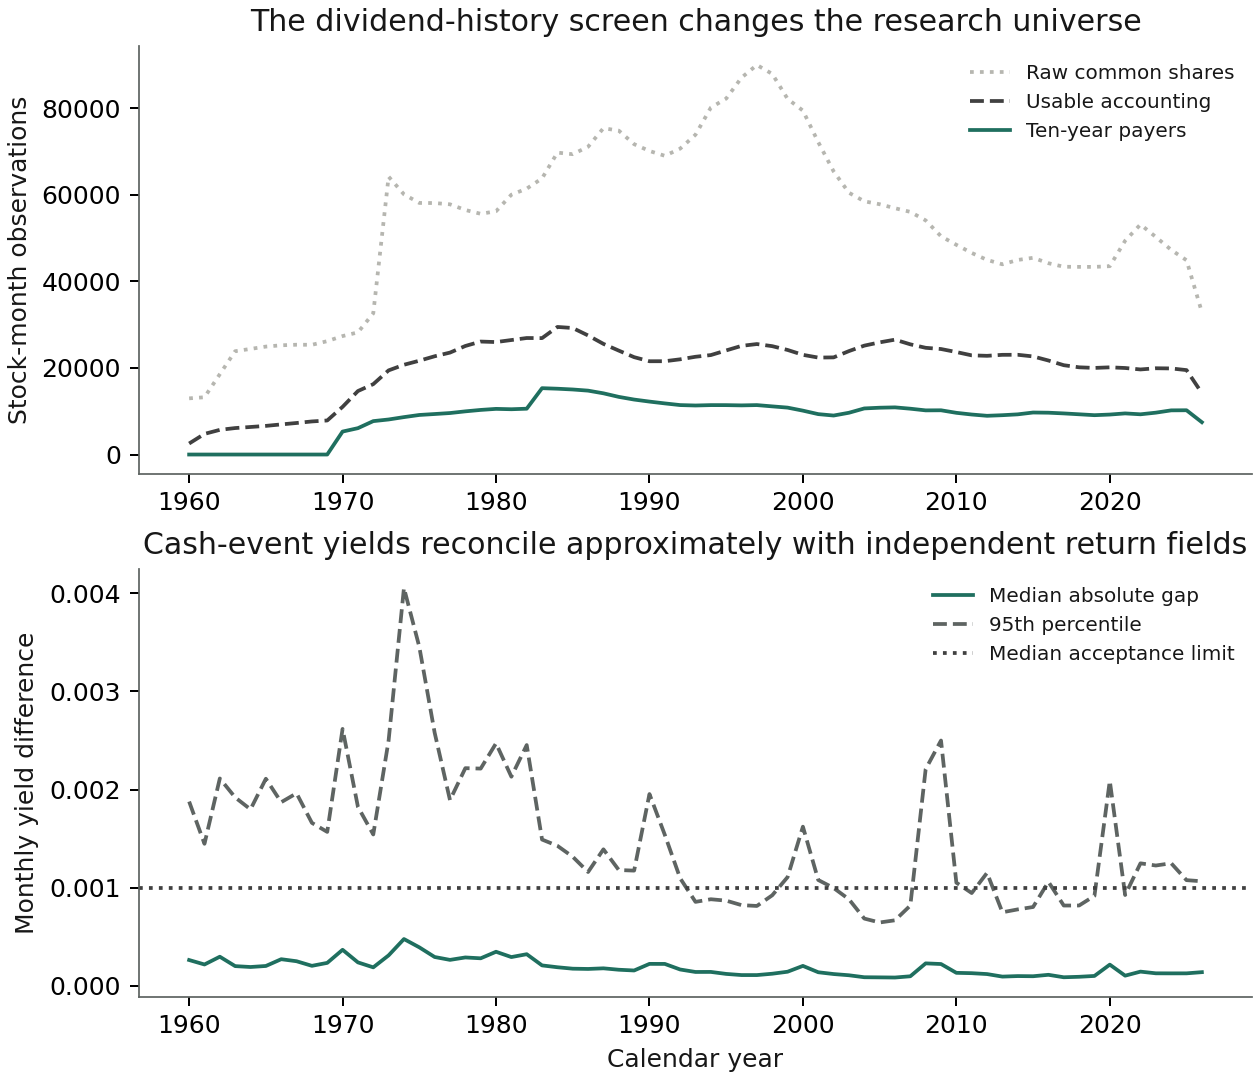
\includegraphics[width=\linewidth,height=.78\textheight,keepaspectratio]{figures/figure_0.png}
\caption{8 of 8 registered checks pass. The median cash-versus-effective yield gap on dividend-paying months is 0.000175; cash withdrawals and daily dividend reinvestment are different conventions. The coverage panel records observed filter attrition, not an assumed target count. A passing identity does not establish exact equivalence to the authors' stock-selection procedure.}\end{figure}


\begin{figure}[p]\centering
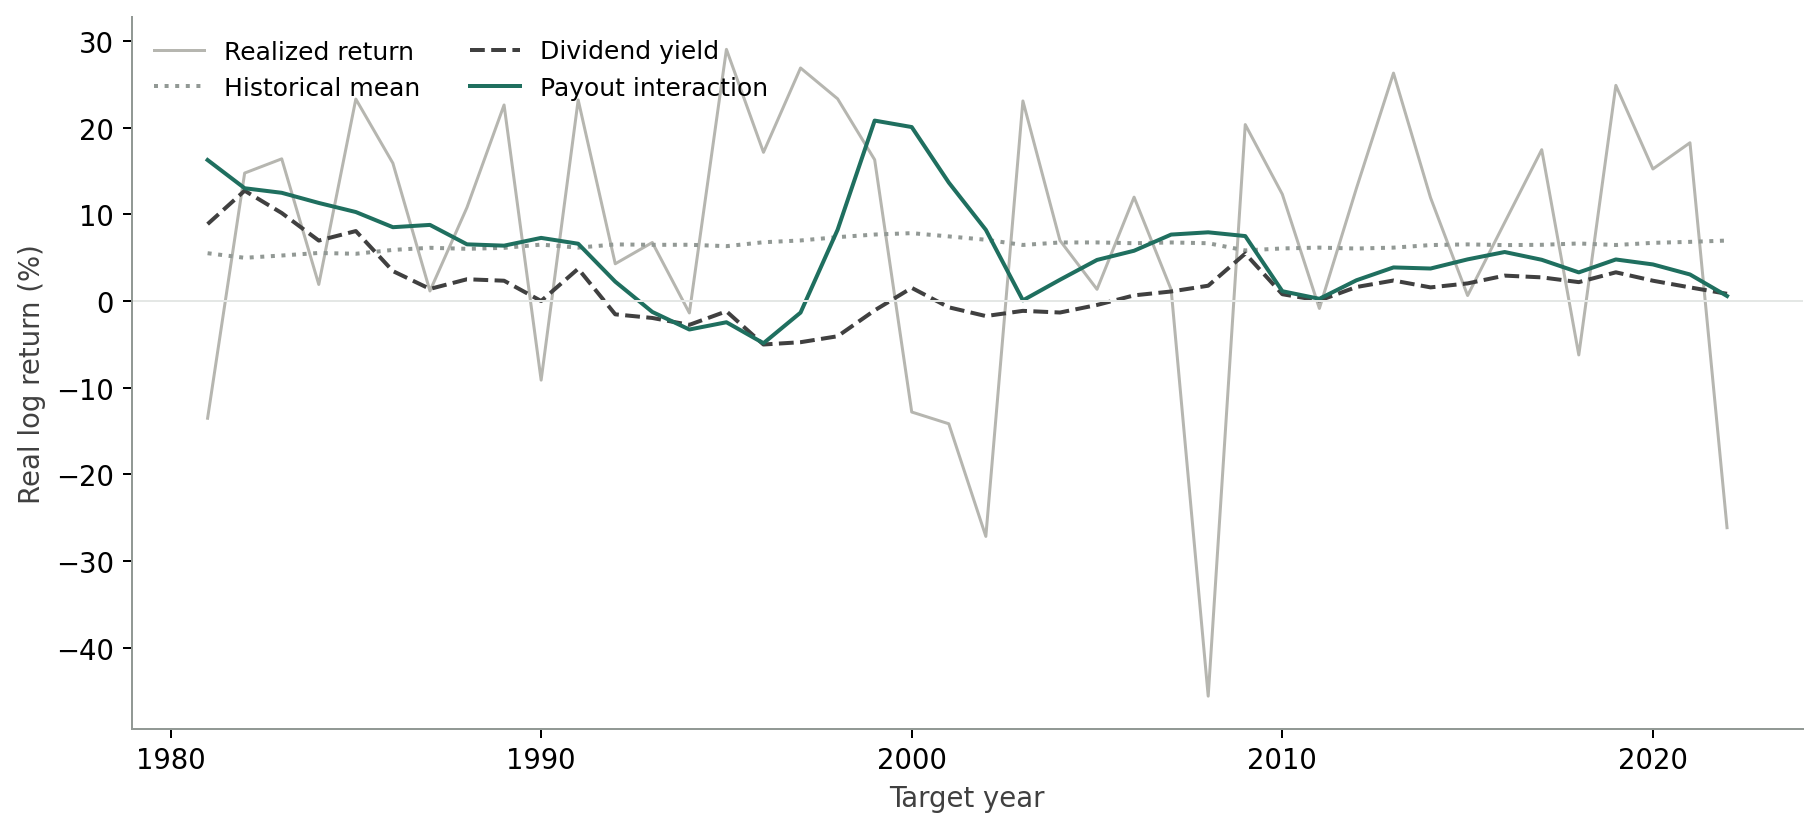
\includegraphics[width=\linewidth,height=.78\textheight,keepaspectratio]{figures/figure_1.png}
\caption{The Historical mean has the lowest out-of-sample RMSE (16.33 log percentage points); the payout-interaction RMSE is 18.28. This legacy exercise does not establish a forecasting improvement from the interaction.}\end{figure}


\begin{figure}[p]\centering
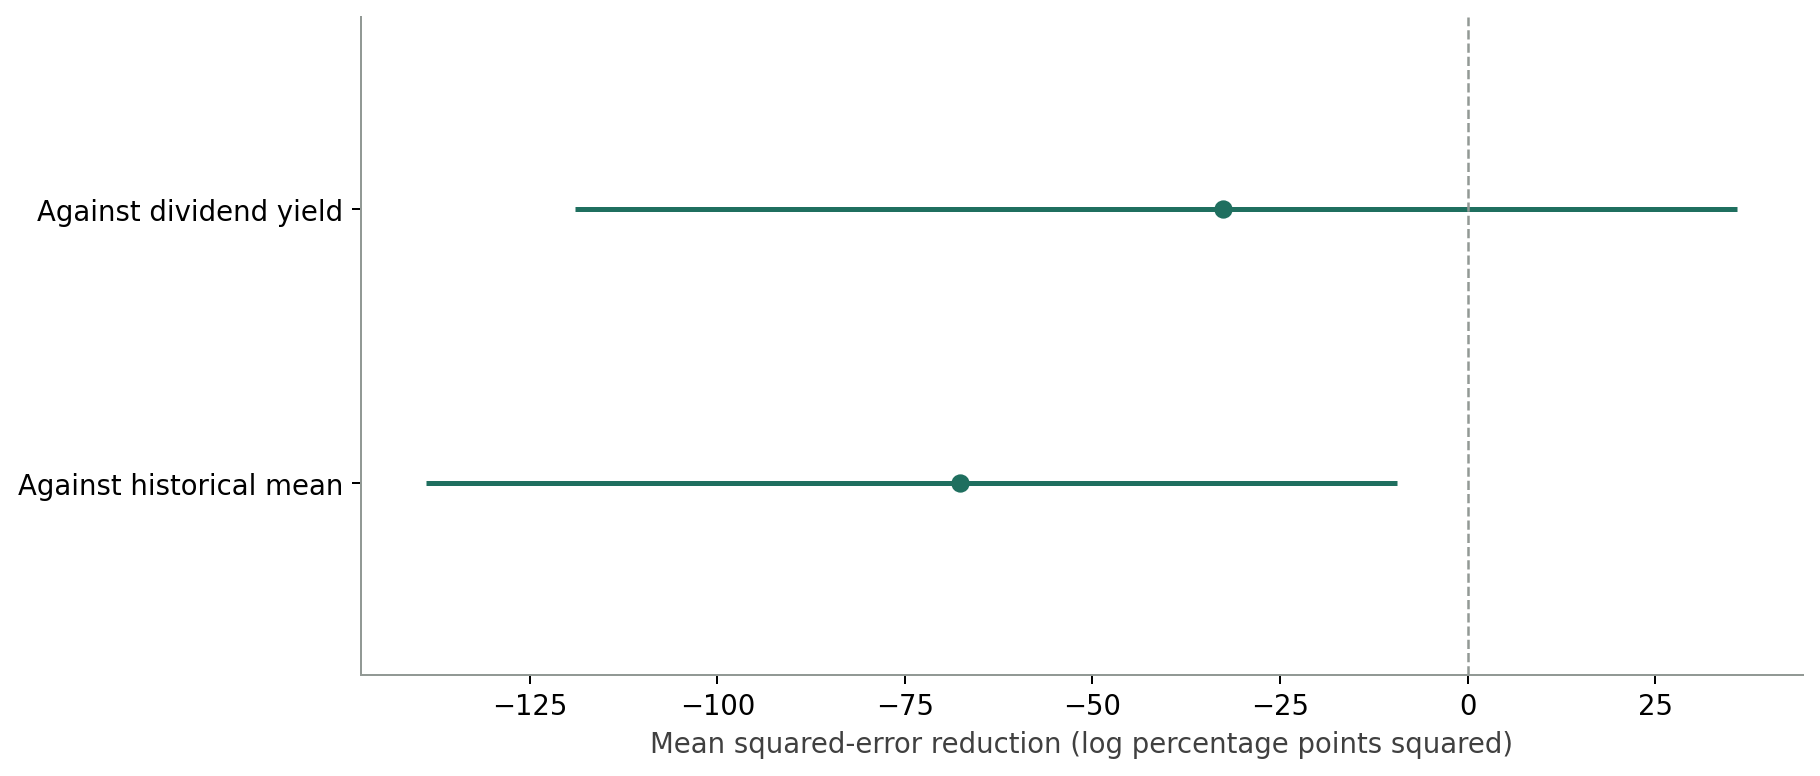
\includegraphics[width=\linewidth,height=.78\textheight,keepaspectratio]{figures/figure_2.png}
\caption{The Historical mean has the lowest out-of-sample RMSE (16.33 log percentage points); the payout-interaction RMSE is 18.28. This legacy exercise does not establish a forecasting improvement from the interaction.}\end{figure}


\begin{figure}[p]\centering
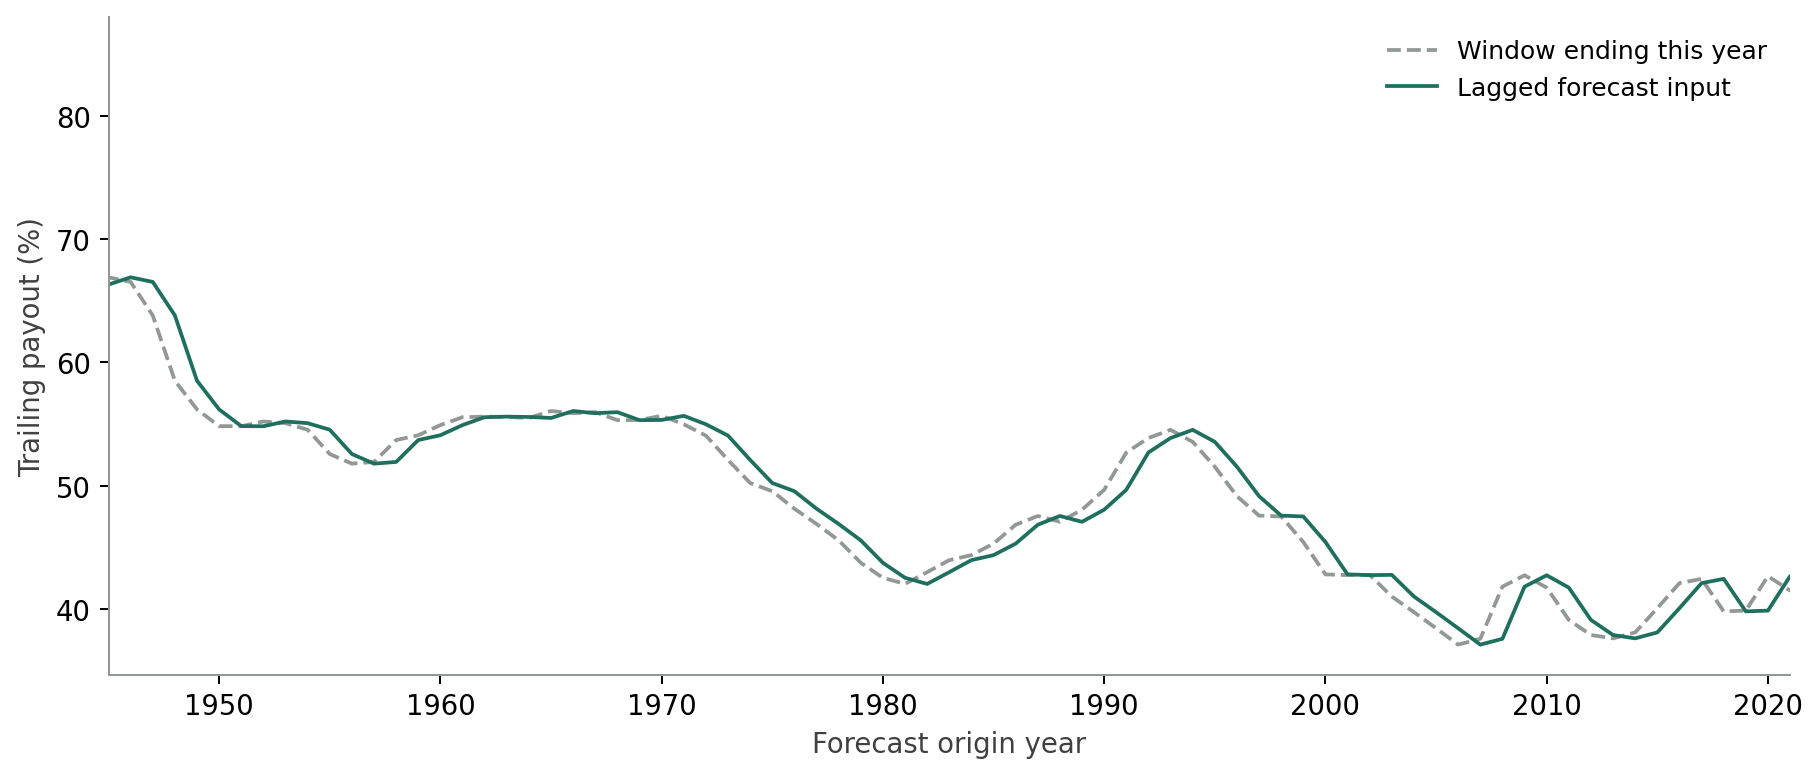
\includegraphics[width=\linewidth,height=.78\textheight,keepaspectratio]{figures/figure_3.png}
\caption{10 of 10 legacy forecast input/timing checks pass. This supports alignment of inputs, not the forecasting value of payout.}\end{figure}


\begin{figure}[p]\centering
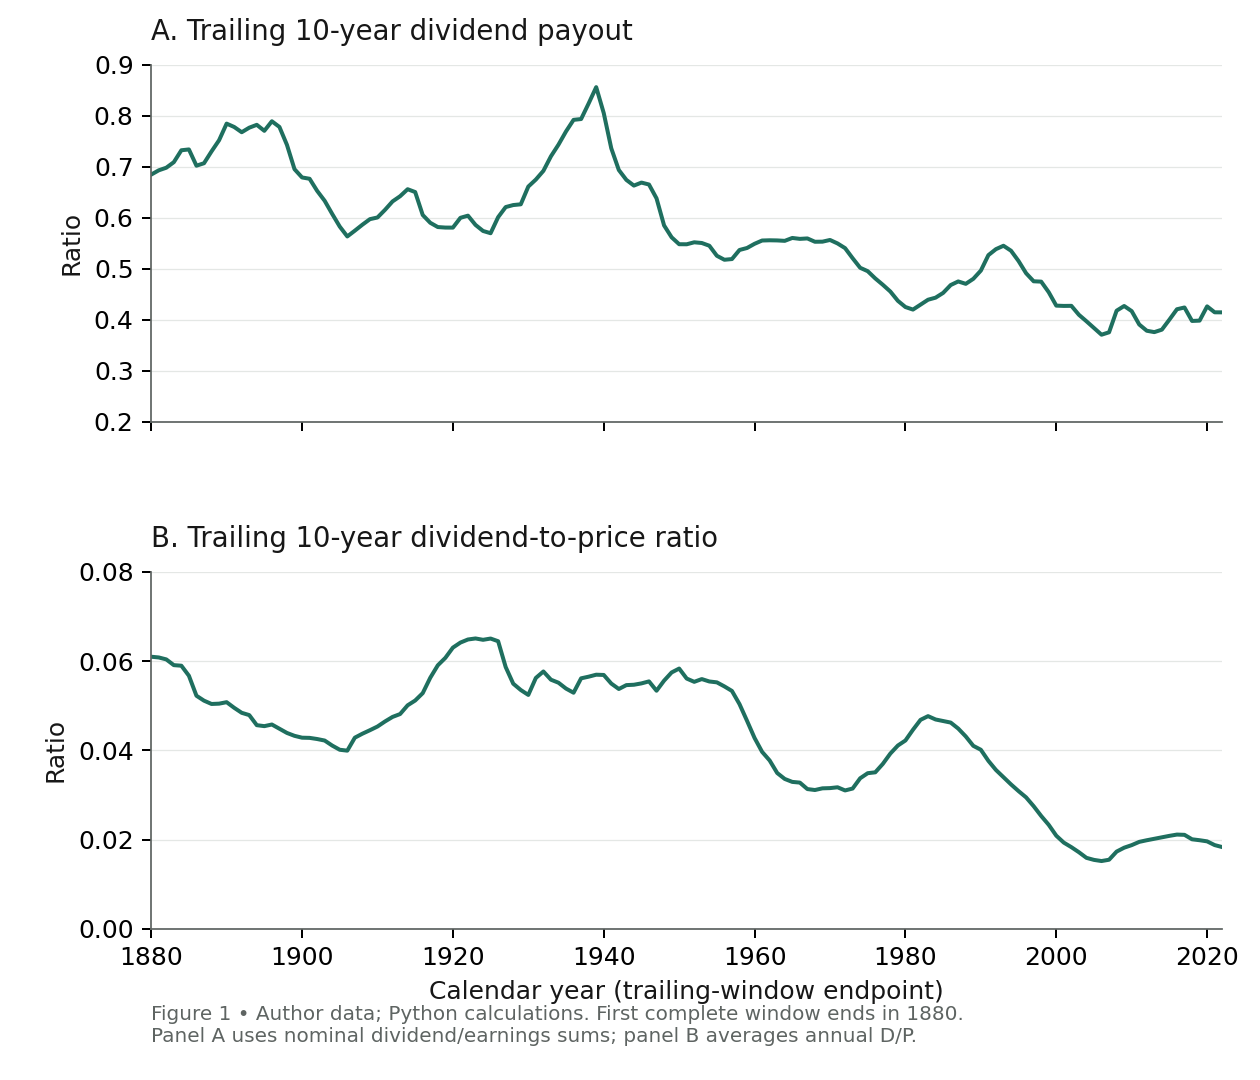
\includegraphics[width=\linewidth,height=.78\textheight,keepaspectratio]{figures/figure_4.png}
\caption{Trailing payout changes from 68.5\% in 1880 to 41.5\% in 2022; trailing D/P changes from 6.1\% to 1.8\%. These endpoint comparisons describe the shift in payouts and valuation.}\end{figure}


\begin{figure}[p]\centering
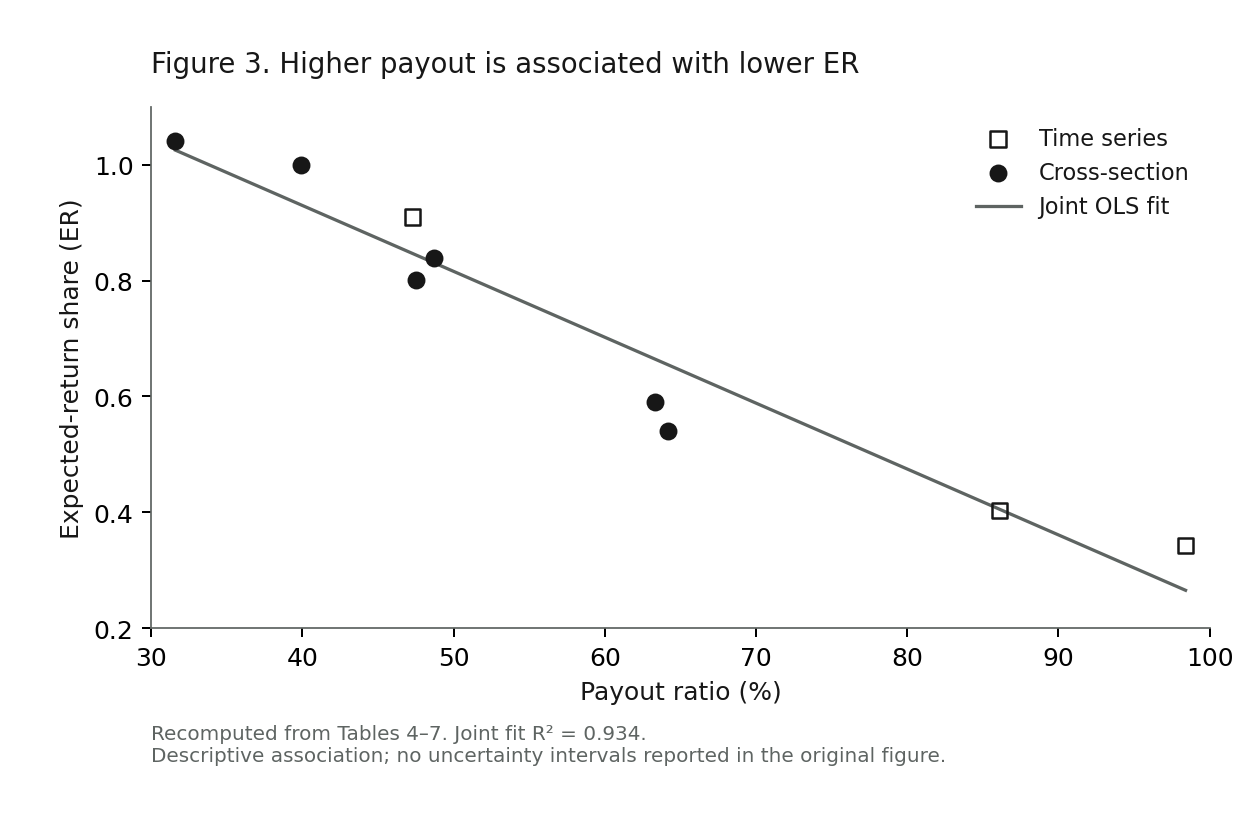
\includegraphics[width=\linewidth,height=.78\textheight,keepaspectratio]{figures/figure_5.png}
\caption{ER ranges from 0.343 to 1.041 across the plotted samples. Payout and ER are compared descriptively; mixed time-series and portfolio points do not identify causation.}\end{figure}


\begin{figure}[p]\centering
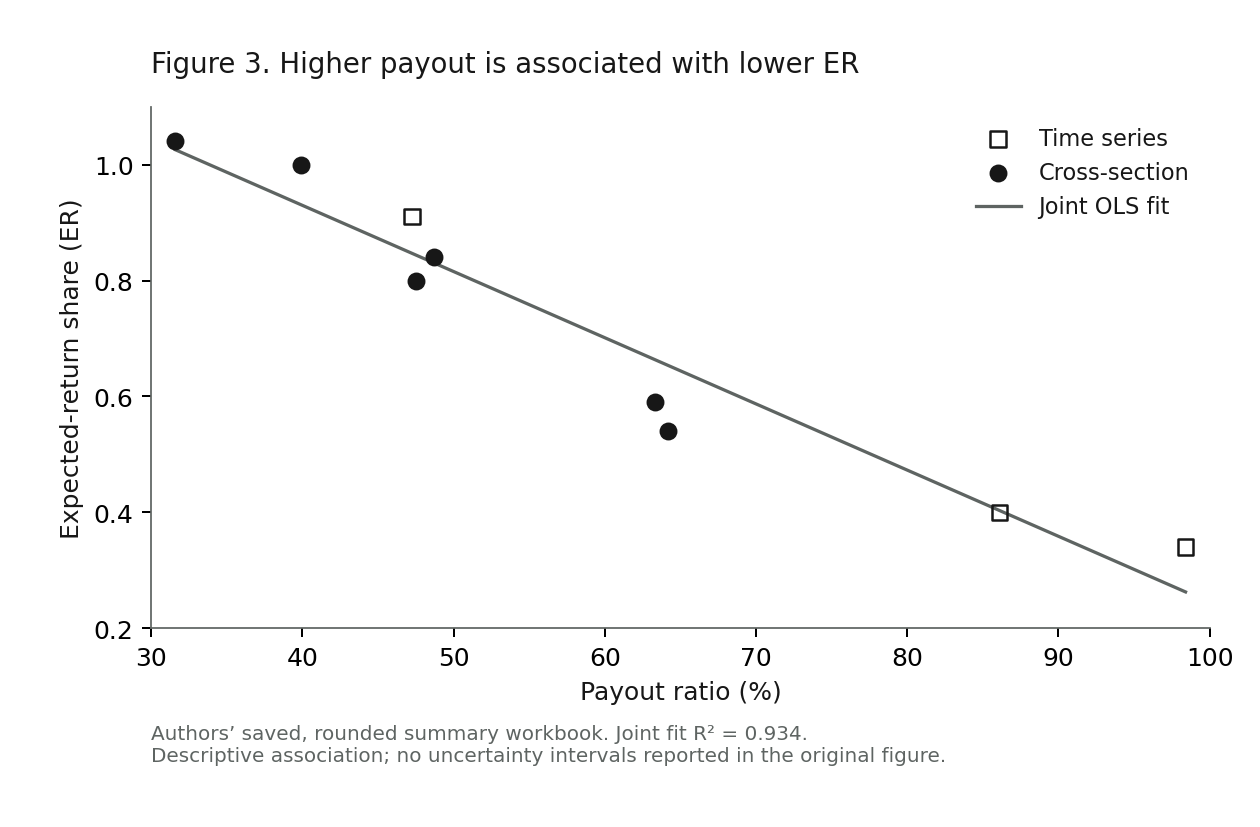
\includegraphics[width=\linewidth,height=.78\textheight,keepaspectratio]{figures/figure_6.png}
\caption{ER ranges from 0.340 to 1.040 across the plotted samples. Payout and ER are compared descriptively; mixed time-series and portfolio points do not identify causation. This is the supplied author-summary sensitivity, not independent numerical replication.}\end{figure}


\begin{figure}[p]\centering
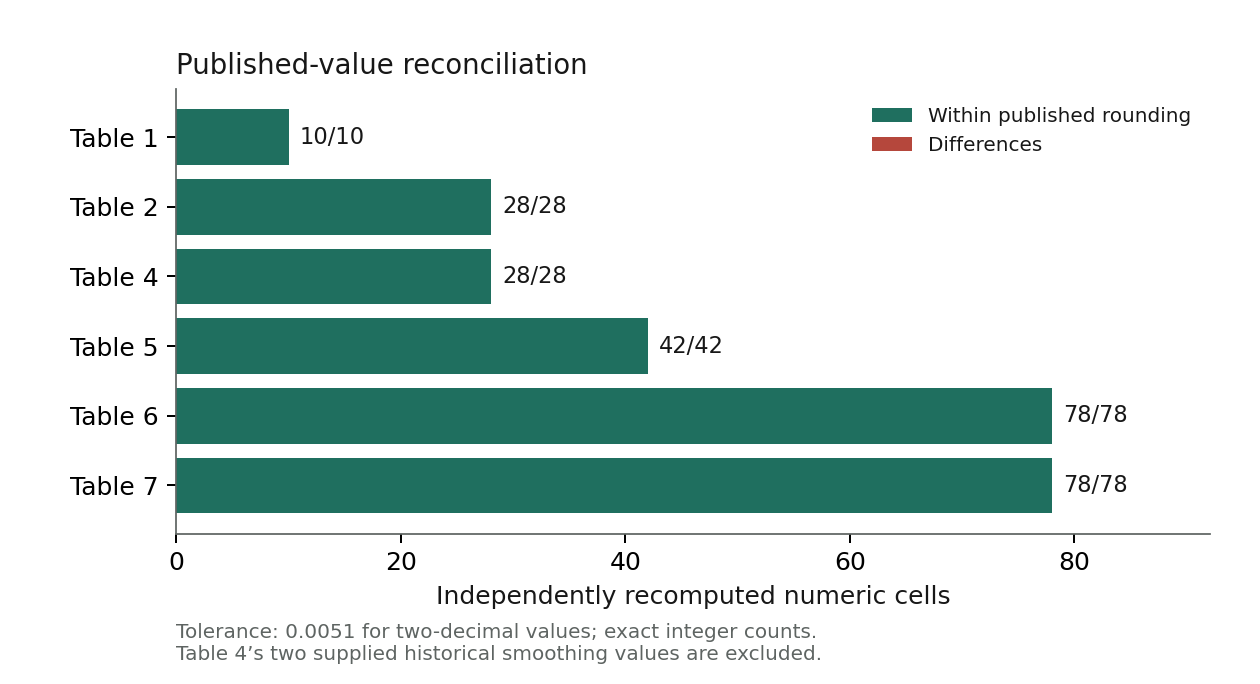
\includegraphics[width=\linewidth,height=.78\textheight,keepaspectratio]{figures/figure_7.png}
\caption{264 independently computed numeric cells meet the published-value tolerance; 2 supplied historical constants remain excluded. Passing the computed cells is not a complete-replication claim.}\end{figure}


\begin{figure}[p]\centering
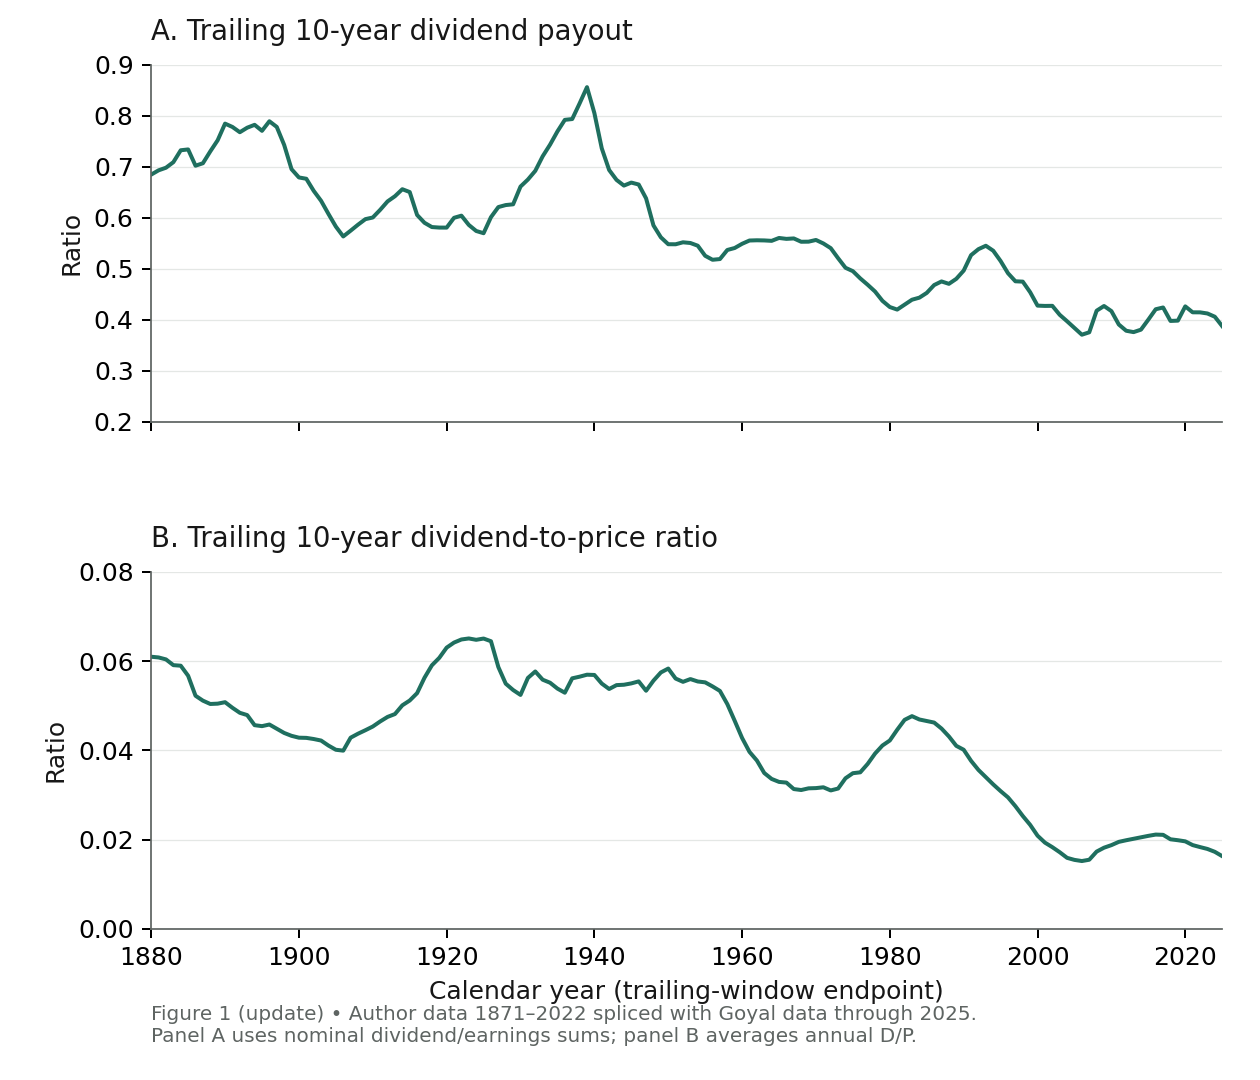
\includegraphics[width=\linewidth,height=.78\textheight,keepaspectratio]{figures/figure_8.png}
\caption{Trailing payout changes from 68.5\% in 1880 to 38.8\% in 2025; trailing D/P changes from 6.1\% to 1.6\%. These endpoint comparisons describe the shift in payouts and valuation.}\end{figure}


\begin{figure}[p]\centering
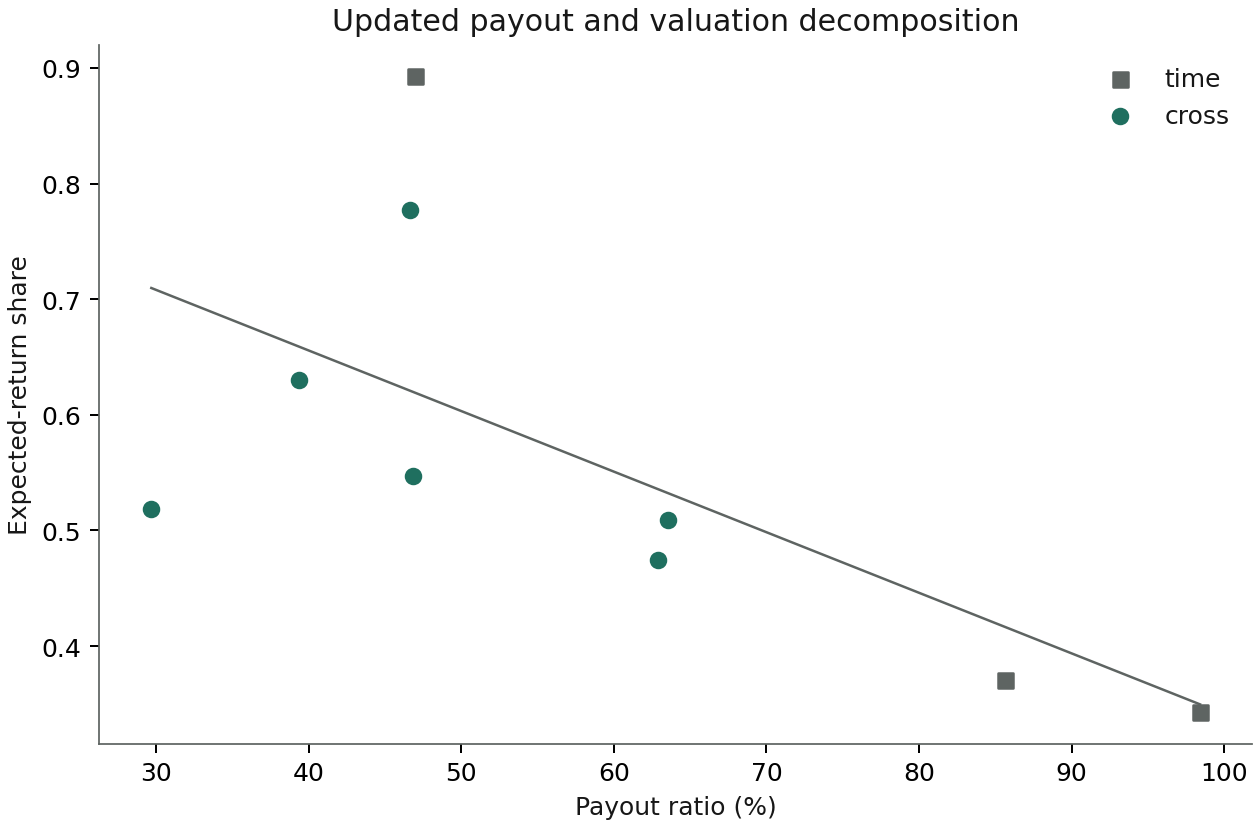
\includegraphics[width=\linewidth,height=.78\textheight,keepaspectratio]{figures/figure_9.png}
\caption{ER ranges from 0.343 to 0.893 across the plotted samples. Payout and ER are compared descriptively; mixed time-series and portfolio points do not identify causation.}\end{figure}


\begin{figure}[p]\centering
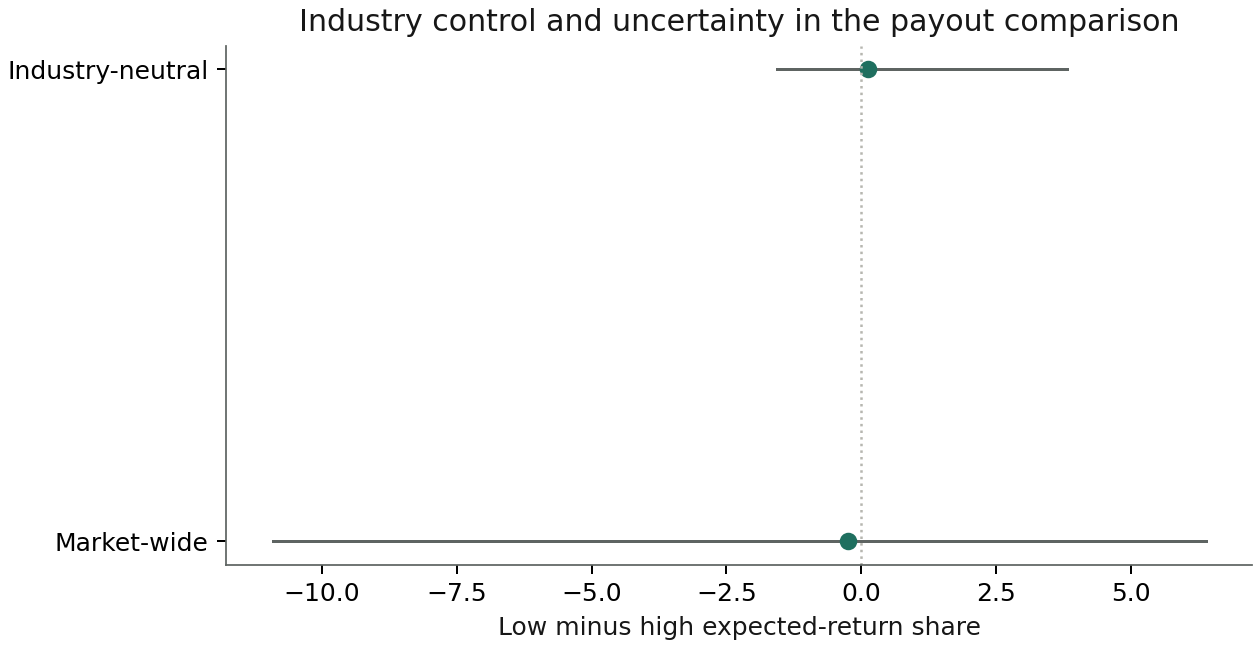
\includegraphics[width=\linewidth,height=.78\textheight,keepaspectratio]{figures/figure_10.png}
\caption{Industry-neutral low-minus-high ER is 0.117, with interval [-1.567, 3.816]. The interval spans zero, so this sample does not establish a payout ordering within industries.}\end{figure}

\clearpage\section{References}Golez, Benjamin, and Peter Koudijs (2025), Equity duration and predictability, Journal of Financial Economics 172, 104114. Replication package: \url{https://doi.org/10.17632/fp6fryn7h3.1}. CRSP methodology and data definitions: \url{https://www.crsp.org/}.\end{document}